\providecommand{\main}{../../..}
\documentclass[\main/dresen_thesis.tex]{subfiles}

\begin{document}
  Maghemite ($\gamma-$\ch{Fe2O3}) and cobalt ferrite (\ch{CoFe2O4}) nanoparticles are nowadays routinely synthesized following methods such as co-precipitation \cite{Fried_2001_Order}, sol-gel \cite{Niederberger_2009_Metal}, micro emulsions \cite{Pillai_1996_Synth}, or thermal decomposition.
  For thermal decomposition, one can further differentiate between hot-injection \cite{Hyeon_2003_Chemi} and heating up methods \cite{Embden_2015_TheHe}.
  Where the first promises monodisperse nanoparticles by keeping the nucleation time period of the synthesis short, the latter is especially promising in being scaleable and highly controllable \cite{Park_2004_Ultra}.
  The heating up method is used extensively in this work to synthesize nanocubes and nanospheres of cobalt ferrite and iron oxide and is further elaborated in the following.

  A popular heating up route to synthesize nanoparticles is to first prepare a metal oleate precursor from metal salts, which is subsequently slowly heated above it's decomposition temperature in a high-boiling solvent, where it is aged in the presence of oleic acid and possibly additional reagents to direct the growth and shape.
  For example, the shape of ferrite nanoparticles can be tuned by adding sodium oleate as precursor before the heating up process.
  The sodium oleate attaches to the (100) facets of forming nanocrystals and fosters the growth along the [111] direction of the crystal \cite{Bao_2009_Forma}.
  By tuning the ratio of sodium oleate to the oleate precursor and adjusting the aging time, this process allows to go from nanospheres over nanocubes to star-shaped nanoparticles.
  Wetterskog \etal extensively studied the formation of maghemite nanospheres and nanocubes during this process \cite{Wetterskog_2014_Preci, Wetterskog_2013_Anoma} and found that due to the reducing environment an antiferromagnetic w\"ustite core is first formed and only by post-synthesis oxidation a maghemite shell is obtained.
  The same can be observed for the synthesis of cobalt ferrite nanoparticles from metal oleates \cite{Bodnarchuk_2009_Excha}, which explains in both cases the low degree of magnetism that is often observed in literature from such synthesis.
  Through forced oxidation after the synthesis the magnetic properties can be enhanced especially for iron oxide nanoparticles.
  However, cobalt ferrite provides a high oxygen diffusion barrier \cite{Chen_2015_Synth} and it is technically harder to oxidize cobalt ferrite nanoparticles completely.

  An alternative heating up synthesis that results in strongly magnetic nanoparticles with pure phase is achieved by the thermal decomposition of metal acetylacetonates in a high boiling solvent such as dibenzyl ether with the presence of oleic acid or oleylamine \cite{Sun_2002_SizeC, Wu_2014_Monol}.
  Again the addition of sodium oleate leads to the formation of nanocubes such as in the oleate synthesis route.
  However, this synthesis is in general difficult to control and scale due to the production of acetone during the synthesis that leads to small but violent explosions at elevated temperatures within the reaction.
  Often the shape of the nanoparticles from this synthesis route is less uniform in comparison to the oleate synthesis route and a lot of fine-tuning and care has to be taken to obtain a good batch of nanoparticles.

  In the following, the preparation of cobalt ferrite nanocubes following both routes is presented and the obtained nanoparticles are characterized similar to \refch{ch:looselyPackedNS}.
  The synthesis and characterization of iron oxide nanocubes following the oleate route is presented in \refch{ch:colloidalCrystals}.

  \subsection{Synthesis from Metal Oleates and Acetylacetonates}
    \subsubsection{Preparation of Cobalt Ferrite Oleate}
      In the first presented protocol to synthesize cobalt ferrite nanoparticles, a cobalt and iron oleate mixture is prepared as first step.
      For this purpose a clear solution of sodium oleate is prepared by dissolving $96 \unit{mmol}$ of \ch{NaOH} in $20 \unit{mL}$ of each \ch{H2O} and \ch{EtOH} and subsequently adding drop wise $96 \unit{mmol}$ of oleic acid under constant stirring.
      Then $12 \unit{mmol}$ of \ch{CoCl2 * 6 H2O} and $24 \unit{mmol}$ of \ch{FeCl3 * 6 H2O} are dissolved $5 \unit{mL}$ \ch{H2O} and $15 \unit{mL}$ \ch{EtOH} each and added to the solution.
      After addition of $80 \unit{mL}$ \ch{H2O} and \ch{EtOH}, as well as $160 \unit{mL}$ n-hexane, the mixture is held at reflux for $4 \unit{h}$ at $60 \unit{^\circ C}$ under constant magnetic stirring.
      Once the mixture is cooled back to room temperature, it is washed three times in a separatory funnel with $30 \unit{mL}$ \ch{H2O} to remove superfluous \ch{NaCl} and the remaining n-hexane, ethanol and water is removed using a rotary evaporator.
      In the end, $31.5 \unit{g}$ of a dark red and highly viscous metal oleate complex is obtained, which is then ready to be used for the nanoparticle synthesis.

    \subsubsection{Preparation of Nanocubes from Oleate}
      To prepare nanoparticles, $10 \unit{mmol}$ of the cobalt ferrite oleate is dissolved in $50 \unit{mL}$ 1-octadecene within a $250 \unit{mL}$ three-neck round-bottom flask.
      To obtain cubically shaped nanoparticles, sodium oleate is prepared by dissolving $2.5 \unit{mmol}$ \ch{NaOH} in $10$ drops of \ch{H2O} and \ch{EtOH} and adding $2.5 \unit{mmol}$ of oleic acid drop wise while ultra sonificating the mixture.
      The sodium oleate is added to the dissolved oleate together with additional $2.5 \unit{mmol}$ oleic acid.
      The mixture is heated and held at $150 \unit{^\circ C}$ for one hour under constant magnetic stirring until all water and ethanol is evaporated.
      A fractionating column is put on the round-bottom flask and nitrogen is gently bubbled into the mixture.
      Using a temperature controller, the mixture is heated to reflux at approx. $315 \unit{^\circ C}$ with a gradient of $2.5 \unit{^\circ C min^{-1}}$, where it is held for $30 \unit{min}$.
      After cooling the reaction naturally to room temperature, the particles are precipitated with \ch{EtOAc} and \ch{EtOH}, centrifuged at $8000 \unit{rpm}$ and redispersed in n-Hexane until the supernatant is clear.
      In the last step the mixture is centrifuged without adding \ch{EtOAc}/\ch{EtOH} and the supernatant fluid is taken as dispersion, where as the precipitate is thrown away as being unstable.
      This synthesis yields approx. $500 \unit{mg}$ nanocubes ($\approx 20 \%$) and is referred to in the following as Ol-CoFe-C.


    \subsubsection{Preparation of Nanocubes from Acetylacetonates}
      To synthesize nanocubes from acetylacetonates, $0.46 \unit{mmol}$ of \ch{Co(acac)2}, $0.8 \unit{mmol}$ of \ch{Fe(acac)3}, $3 \unit{mmol}$ of freshly prepared sodium oleate and $3 \unit{mmol}$ of oleic acid are diluted in $10 \unit{mL}$ of dibenzyl ether in a $50 \unit{mL}$ three-neck round-bottom flask.
      The mixture is heated to $120 \unit{^\circ C}$ and held here for $1 \unit{h}$.
      After putting a fractionating column on the round-bottom flask and, a temperature controller is used to heat the mixture to reflux at about $290 \unit{^\circ C}$ with a heating rate of $10 \unit{^\circ C min^{-1}}$.
      During the synthesis, nitrogen is blown gently into the solution all the time and the solution is magnetically stirred.
      After cool down, the product is transferred with n-Hexane to centrifugal tubes and precipitated with \ch{EtOH}.
      After centrifugation at $8500 \unit{rpm}$ the supernatant is thrown away and the precipitate is redispersed with n-Hexane .
      This procedure is repeated three times and in the last step the precipitate is dispersed in n-Hexane without precipitating it again.
      After a final centrifugation at $8500 \unit{rpm}$ the supernatant is kept as product.
      The synthesis yields approx. $50 \unit{mg}$ nanocubes ($\approx 45 \%$) and is referred to in the following as Ac-CoFe-C.

  \subsection{Structural Characterization of the Nanocubes}
  \label{sec:monolayers:nanoparticle:structuralCharacterization}
    After synthesis, transmission electron microscopy is used to characterize a sample of the prepared dispersion and validate the structural quality of the batch.
    The exemplary images shown in \reffig{fig:monolayers:nanoparticle:tem} reveal that both procedures result in nanocubes.
    The particles from the metal oleate (Ol-CoFe-C) are qualitatively more homogeneous in shape than the particles from acetylacetonates (Ac-CoFe-C) and have an average edge length of $10.90(4) \unit{nm}$ with size distribution $8.8(3) \unit{\%}$.
    Within Ac-CoFe-C, some corners of the cubes are not completely developed and non-cubic particles can be found in between the cubes, their average edge length is estimated to $10.8(1) \unit{nm}$ with size distribution $9.9(8) \unit{\%}$.

    \begin{figure}[tb]
      \centering
      \hspace{0.3 cm}
      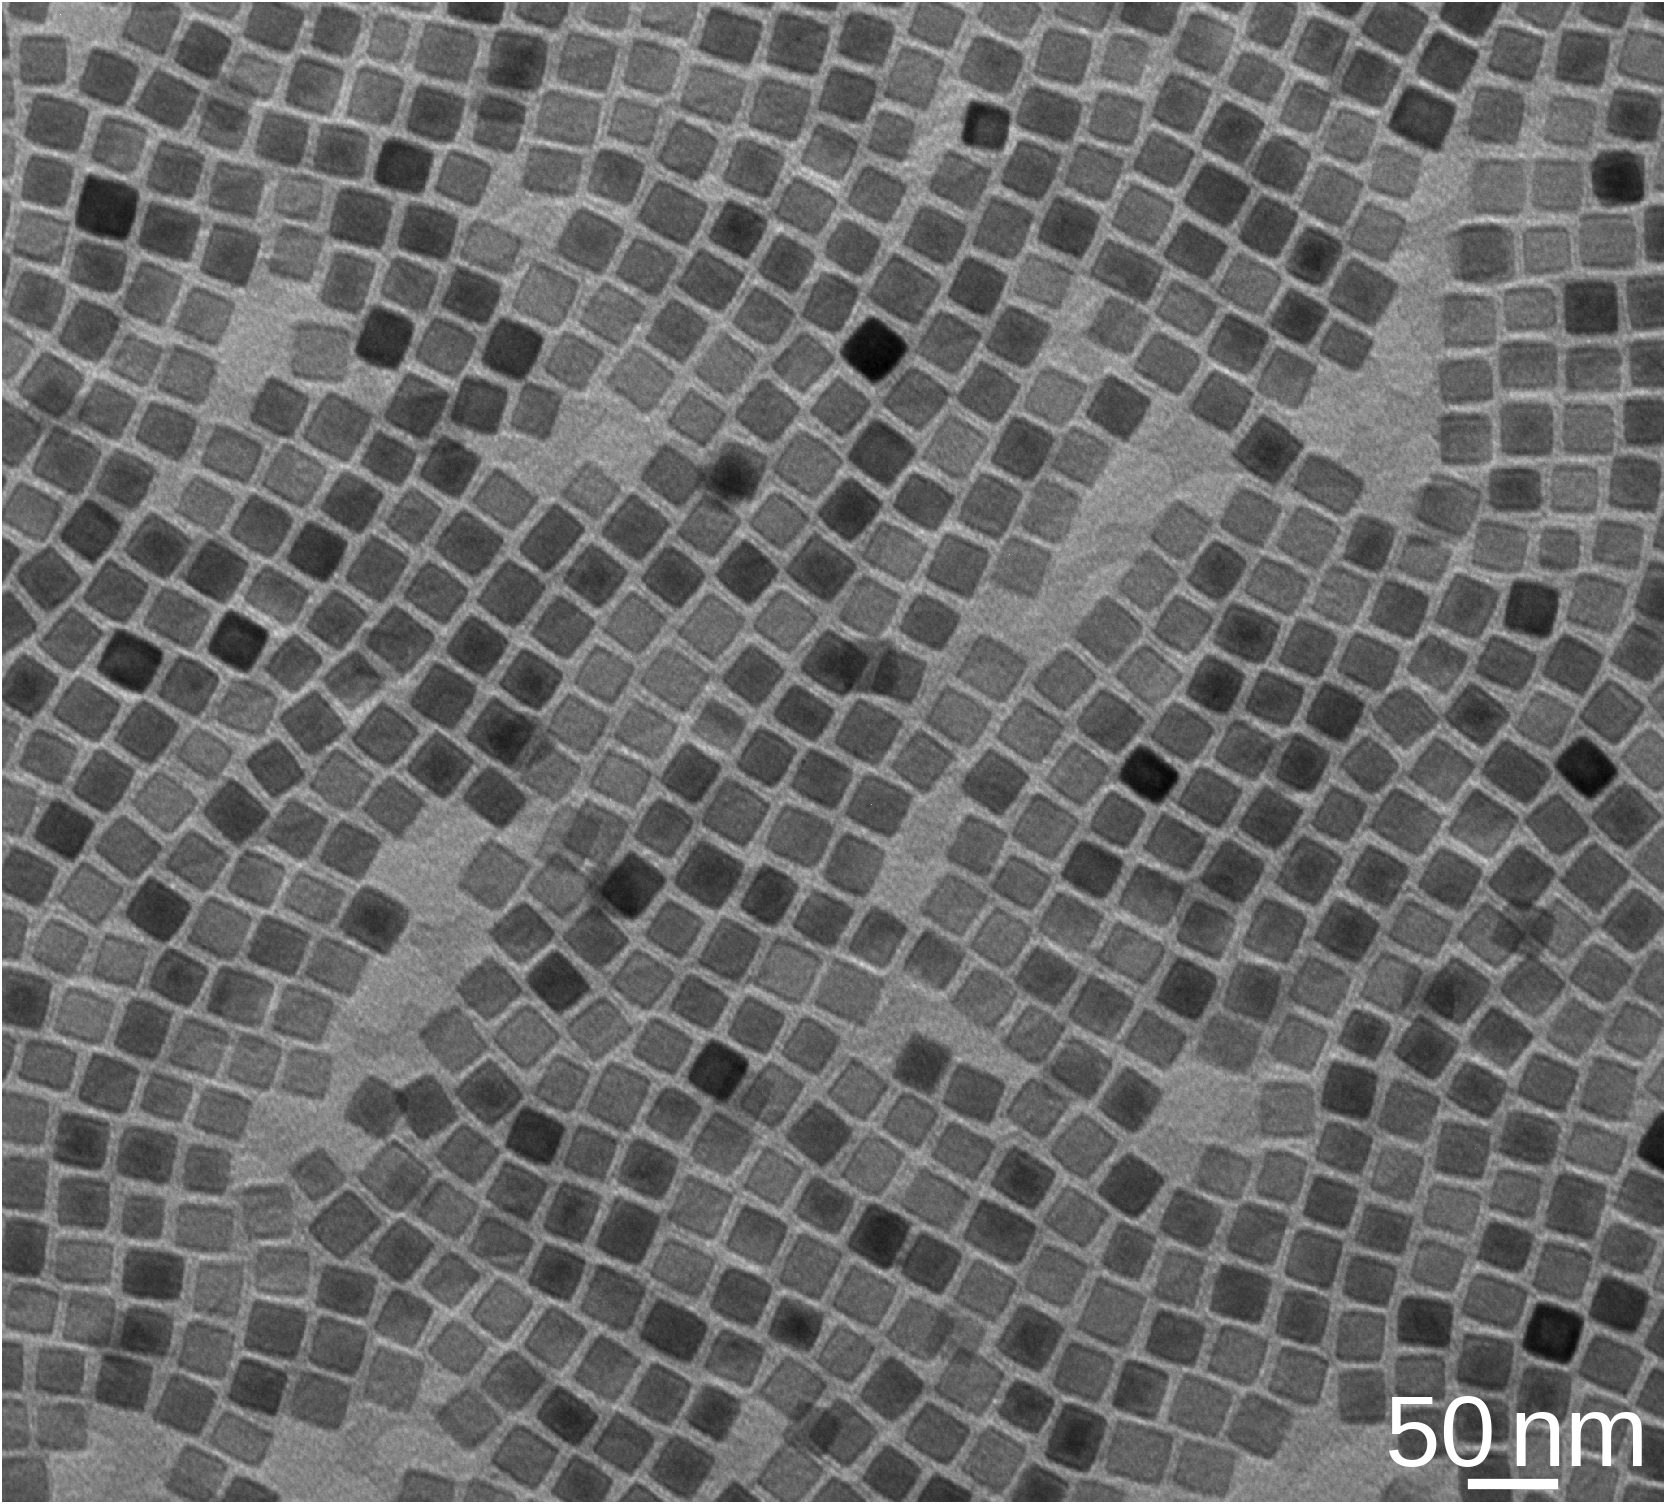
\includegraphics{monolayers_TEM_Ol_CoFe_C}
      \hspace{0.3 cm}
      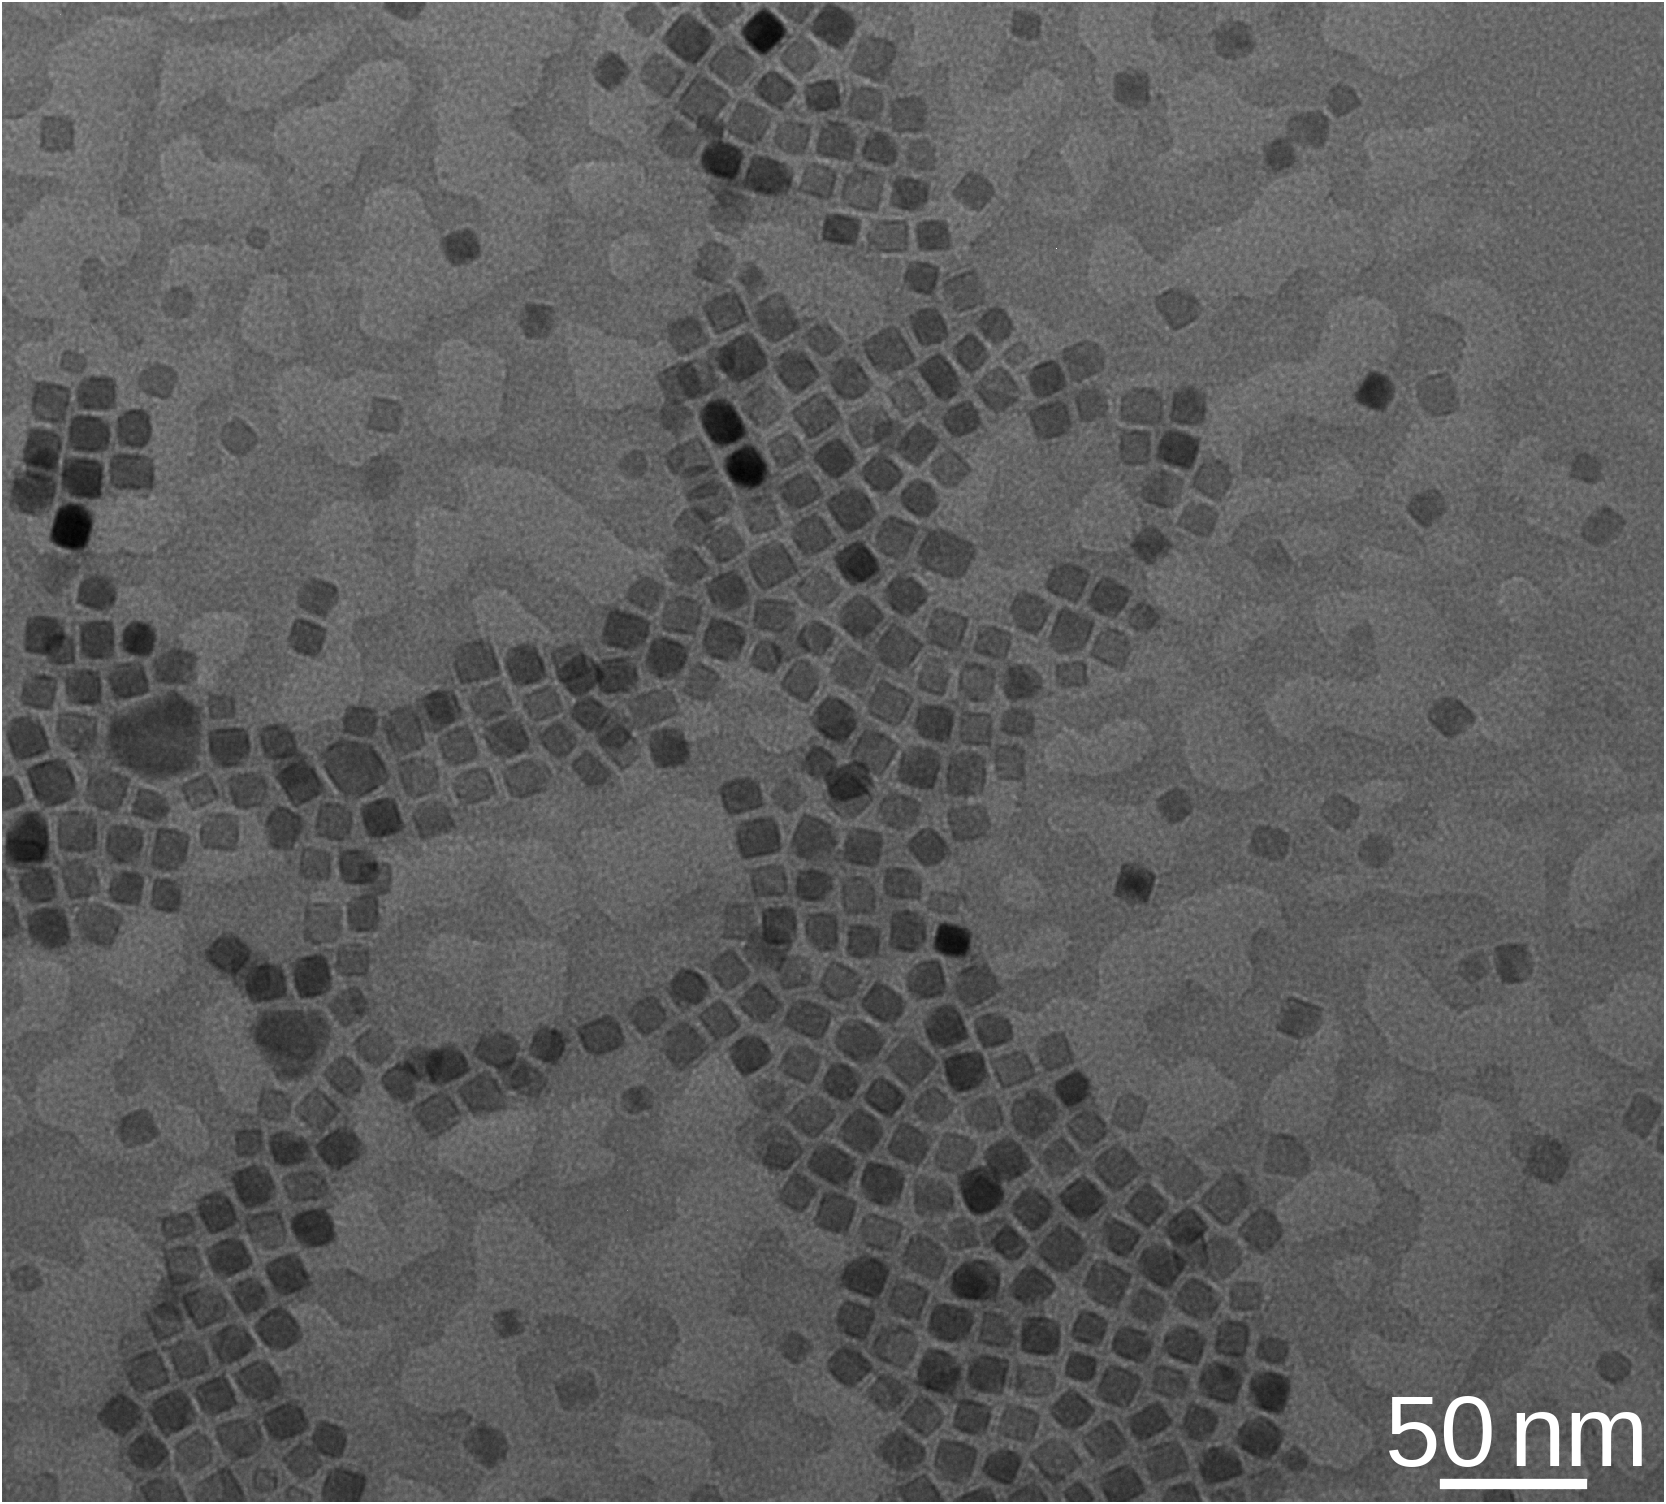
\includegraphics{monolayers_TEM_Ac_CoFe_C}
      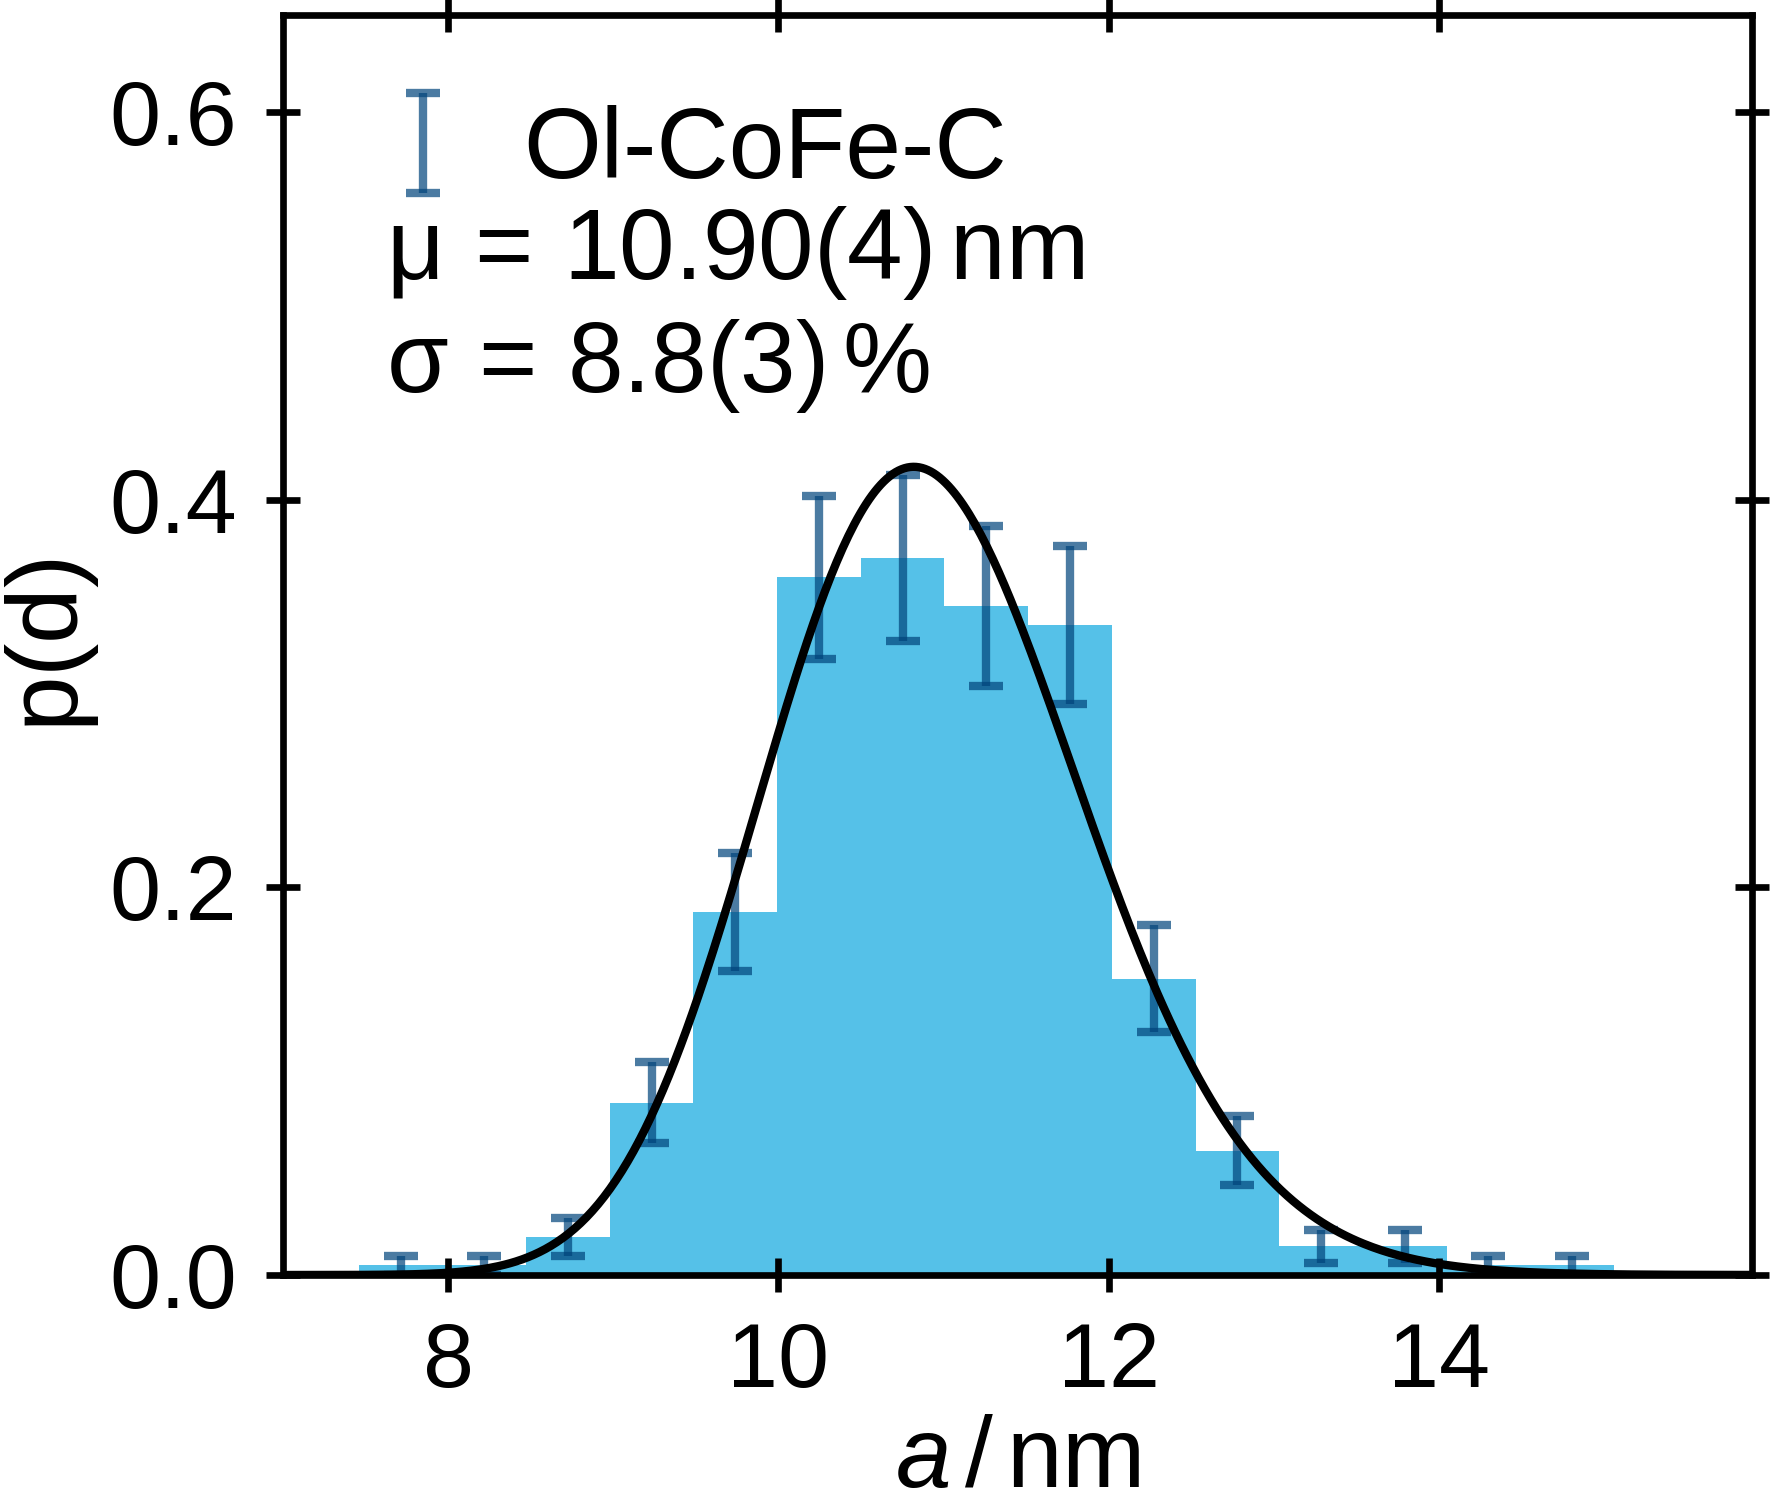
\includegraphics{monolayers_TEM_Ol_CoFe_C_sizeDist}
      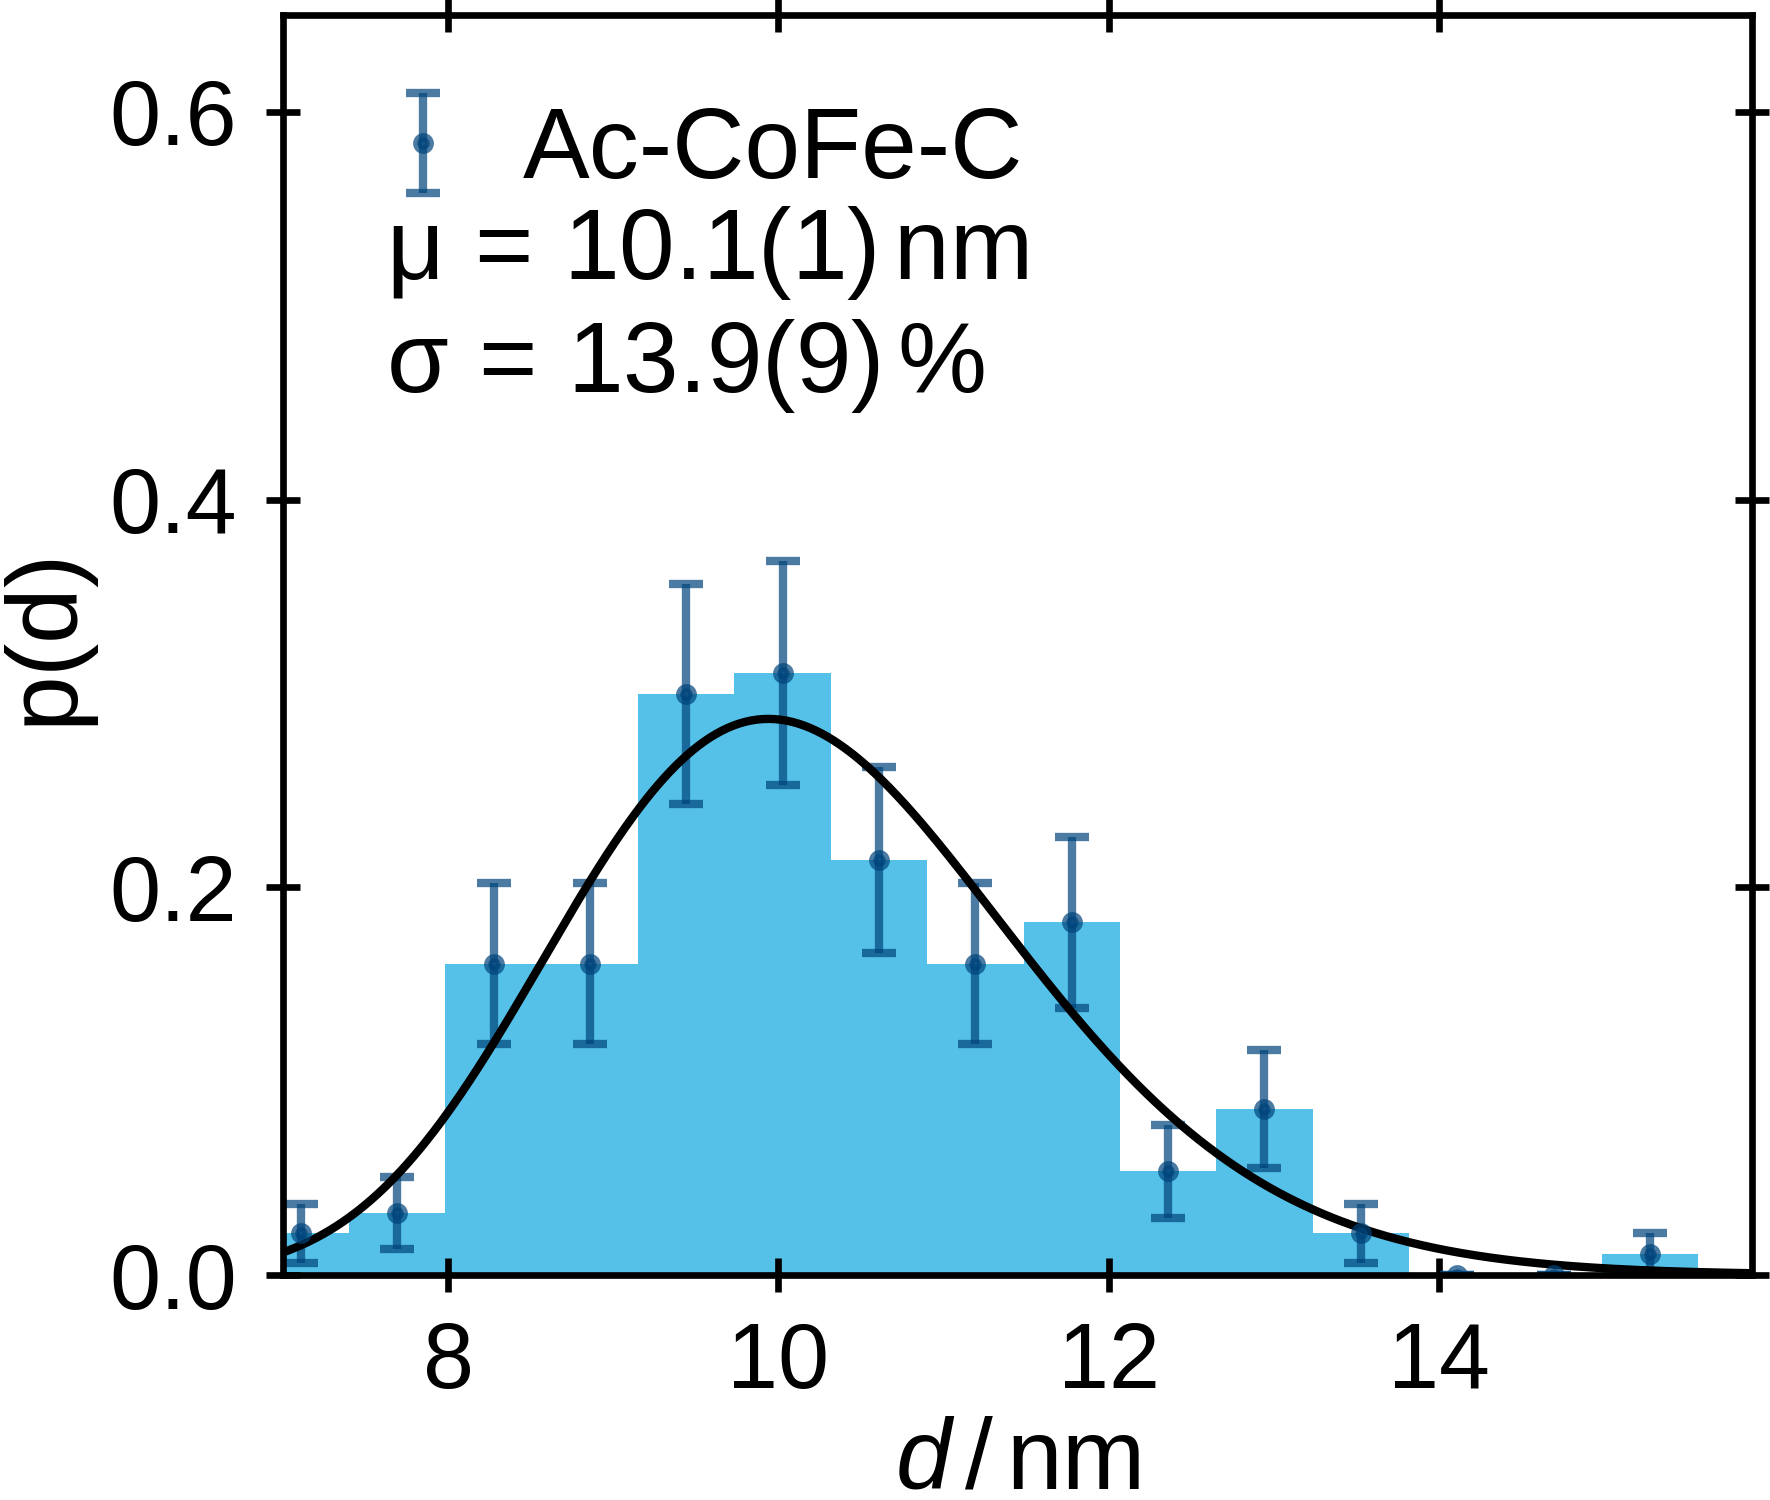
\includegraphics{monolayers_TEM_Ac_CoFe_C_sizeDist}
      \caption{\label{fig:monolayers:nanoparticle:tem}Transmission electron microscopy images of cobalt ferrite nanocubes synthesized from oleates (upper left) and acetylacetonates (upper right) and the edge length size distribution evaluated from the images below respectively.}
    \end{figure}

    Using small-angle x-ray and neutron scattering, the nuclear and magnetic structure of diluted nanoparticles in dispersion is quantitatively evaluated over a macroscopic area of the sample and shown in \reffig{fig:monolayers:nanoparticle:sas:AcOlCoFeC}.
    For the SAXS measurement, the sample were diluted in n-hexane and measured at the GALAXI instrument in the Forschungszentrum J\"ulich, which is described in \refapp{ch:appendix:lss:galaxi}.
    The small angle neutron scattering data was measured using the D33 instrument at the Institut Laue-Langevin, which is described in \refapp{ch:appendix:lss:d33}.
    For the neutron scattering experiment, the sample was dispersed in deuterated toluene to reduce the incoherent scattering coming from hydrogen atoms.
    The comparison between the Ol-CoFe-C and Ac-CoFe-C small angle scattering data shows on a qualitative level that the nanocubes synthesized following the oleate route have a smaller size distribution and higher homogeneous sample quality as more oscillations are visible with more pronounced minima.
    However, it also shows that Ol-CoFe-C is only weakly magnetic whereas the particles in Ac-CoFe-C have a stronger magnetic moment, which is visible in the greater splitting of $I(+)$ and $I(-)$ in SANSPOL.

    \begin{figure}[tb]
      \centering
      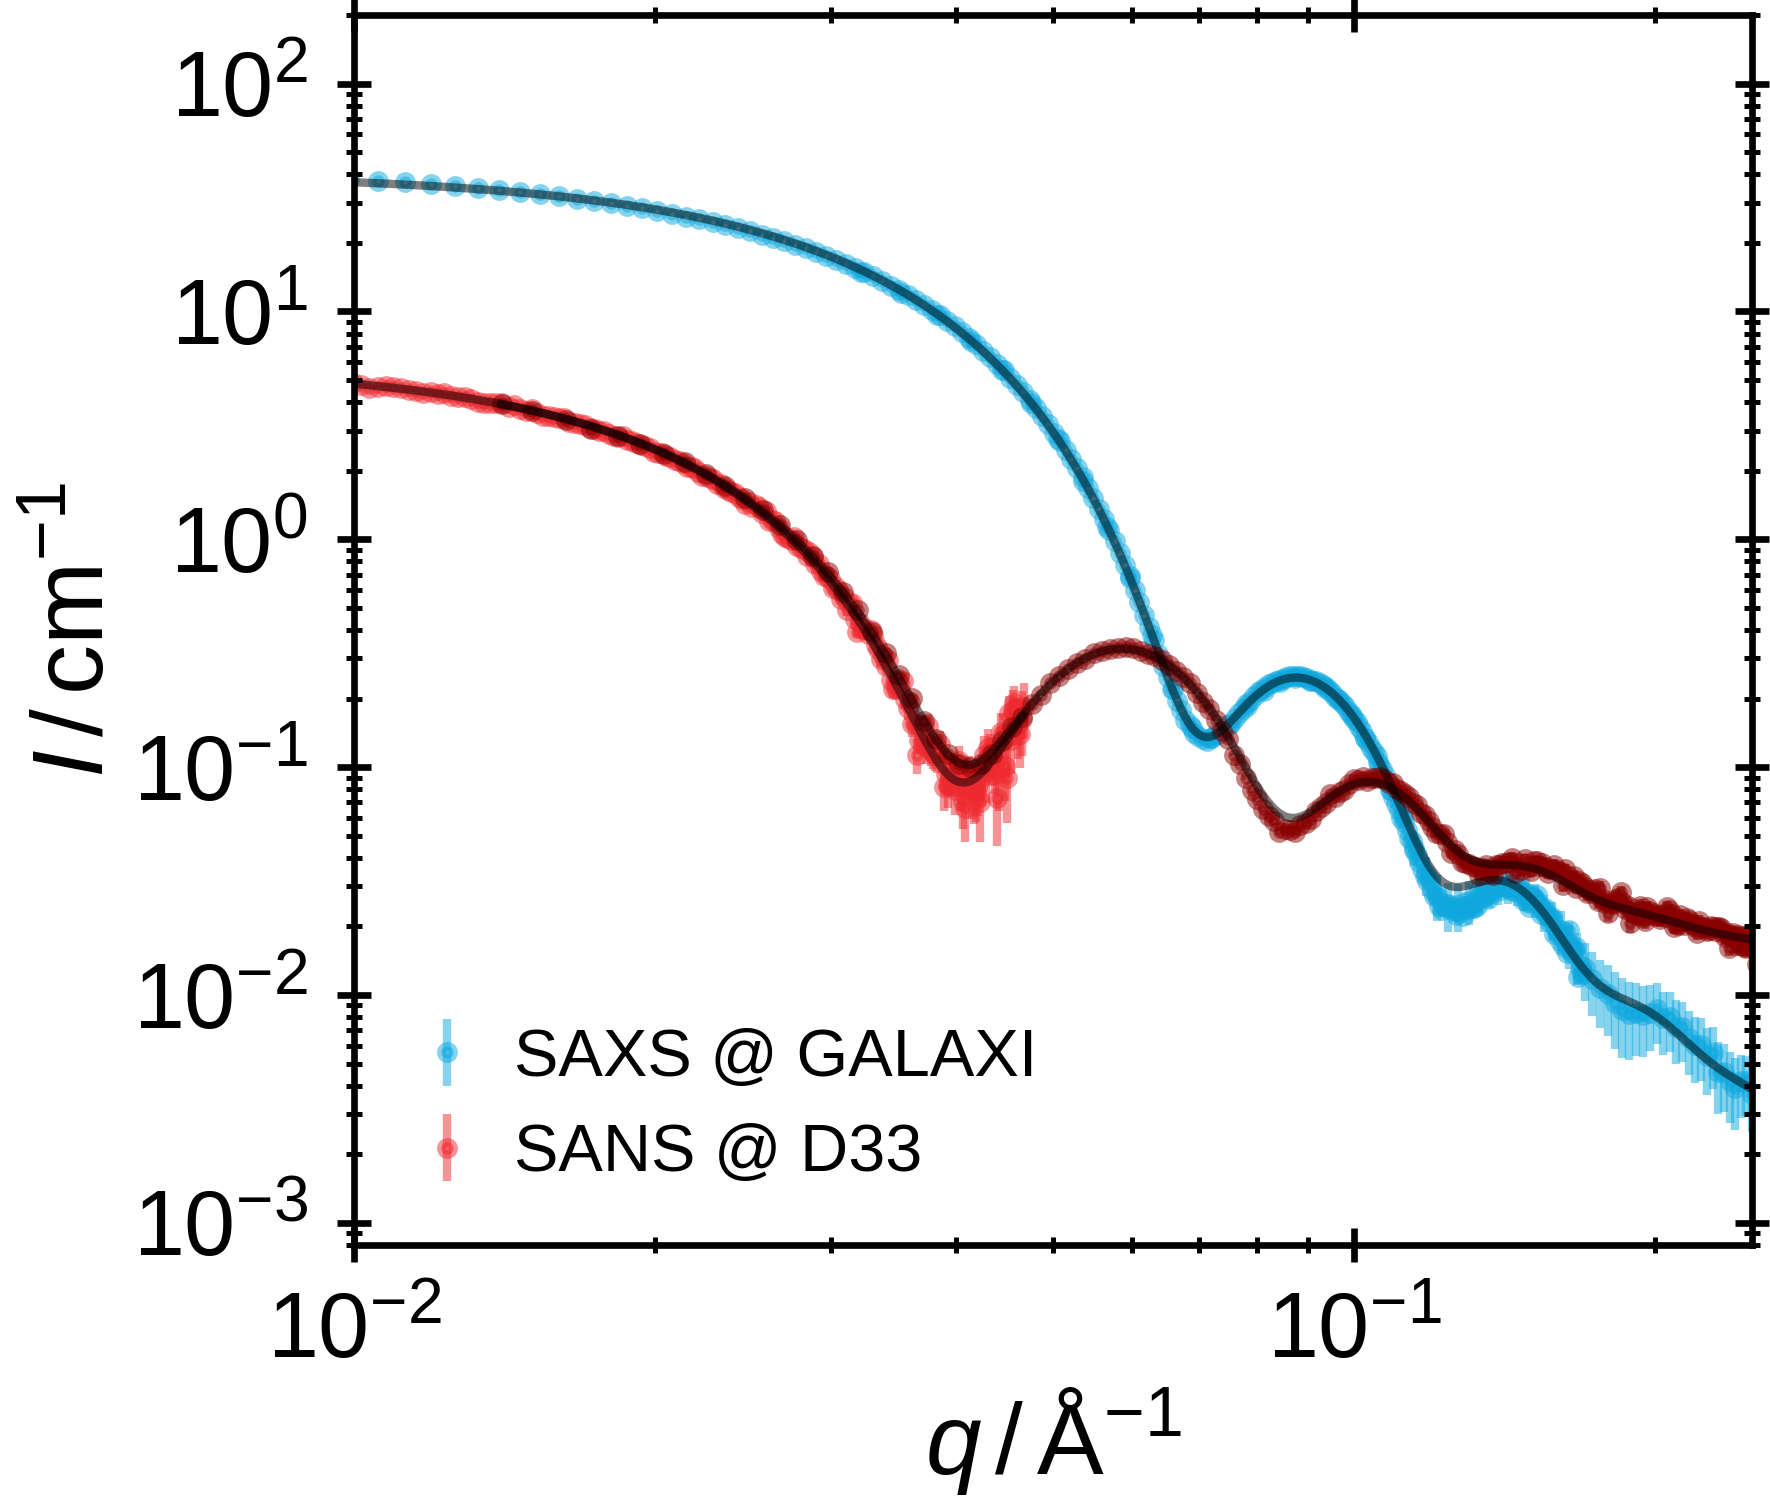
\includegraphics{monolayers_SAS_Ol_CoFe_C_SASFit}
      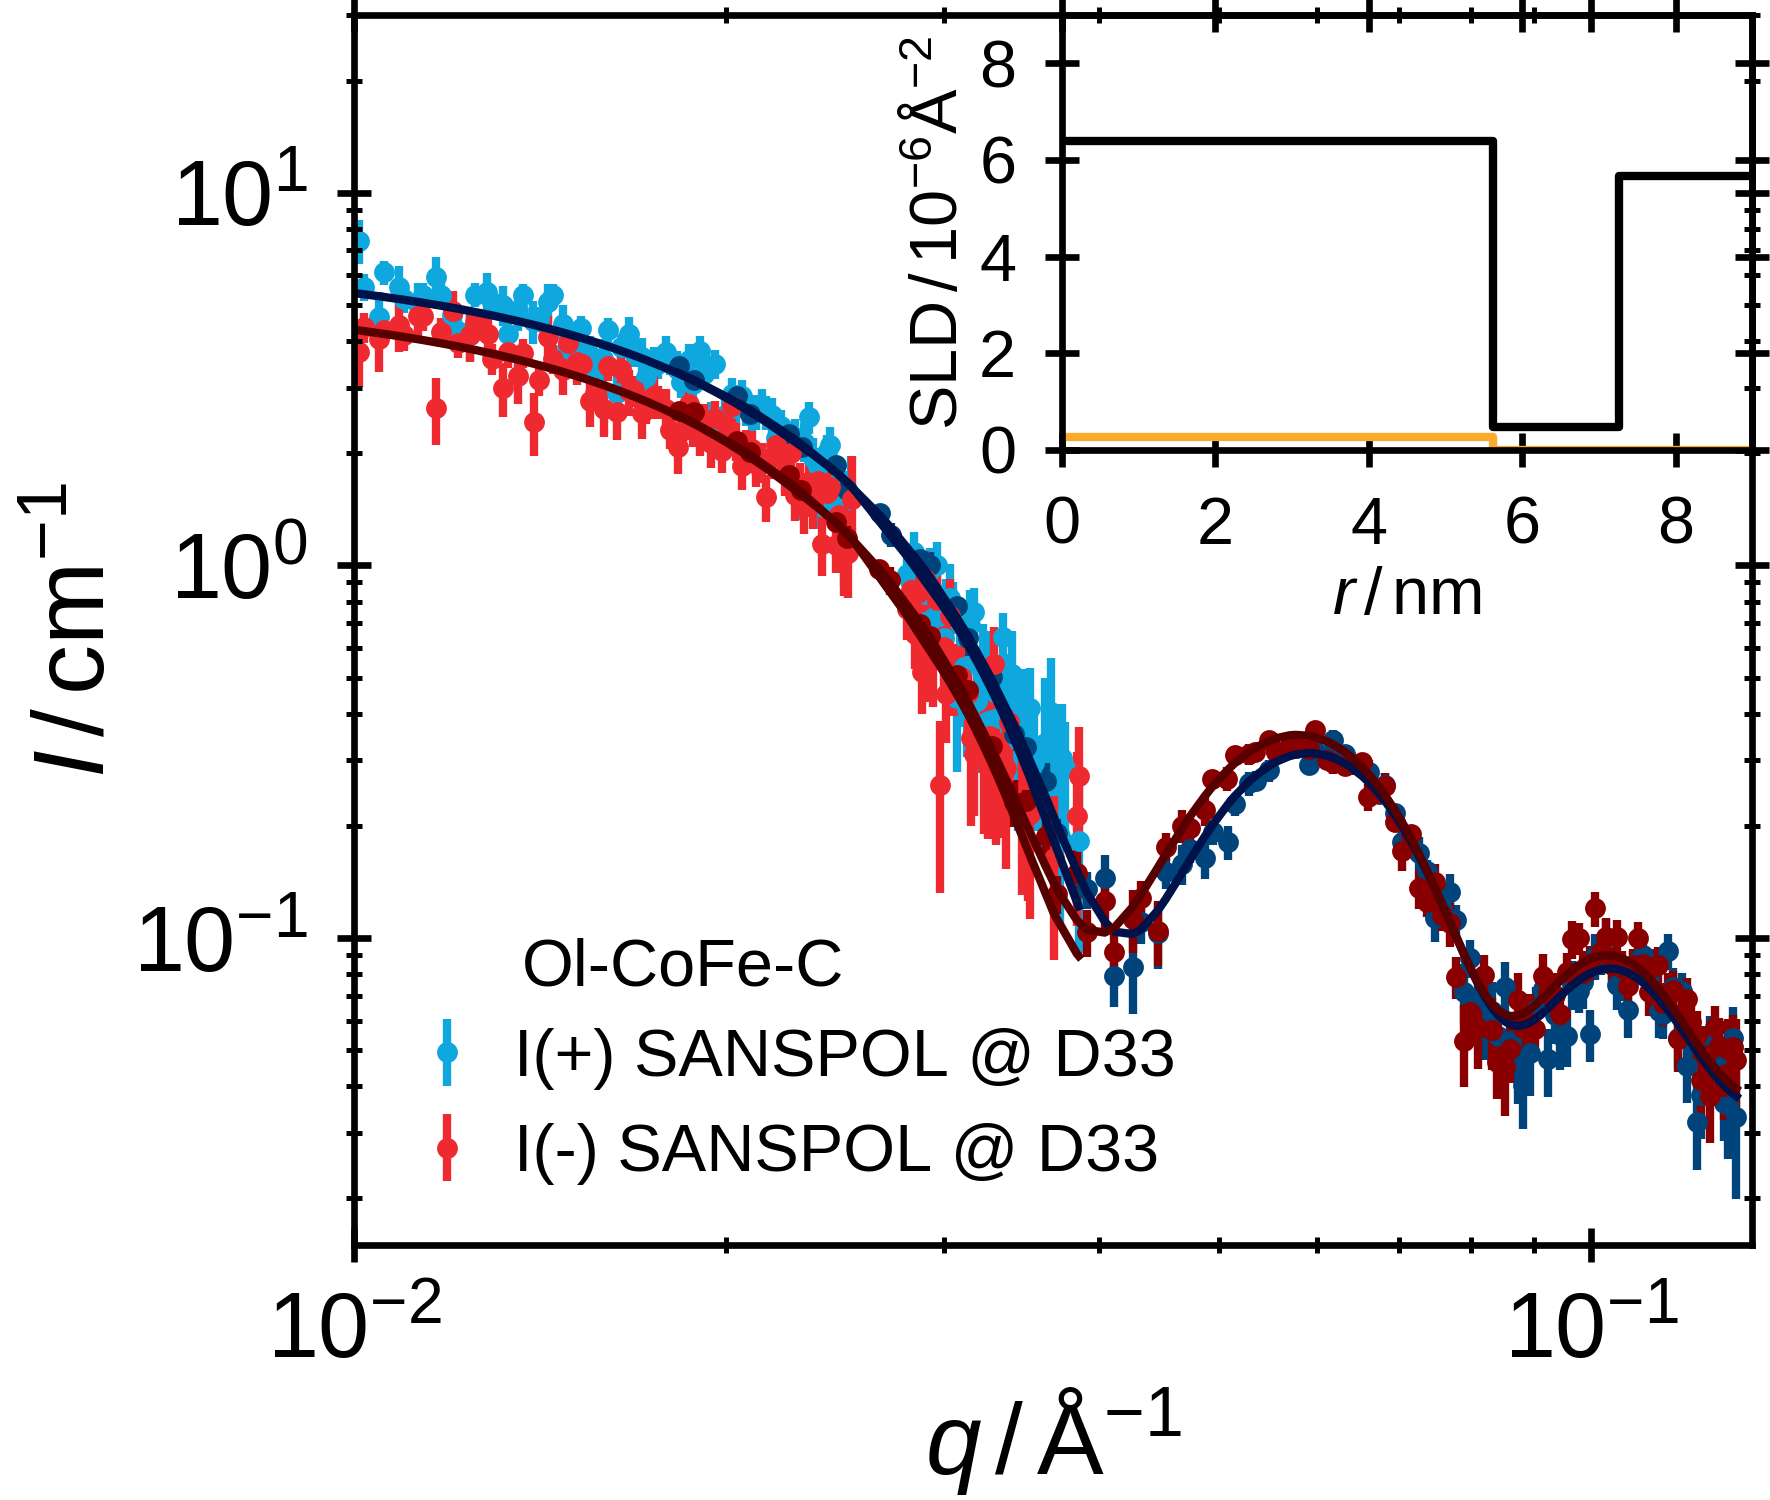
\includegraphics{monolayers_SAS_Ol_CoFe_C_SANSPOLFit}
      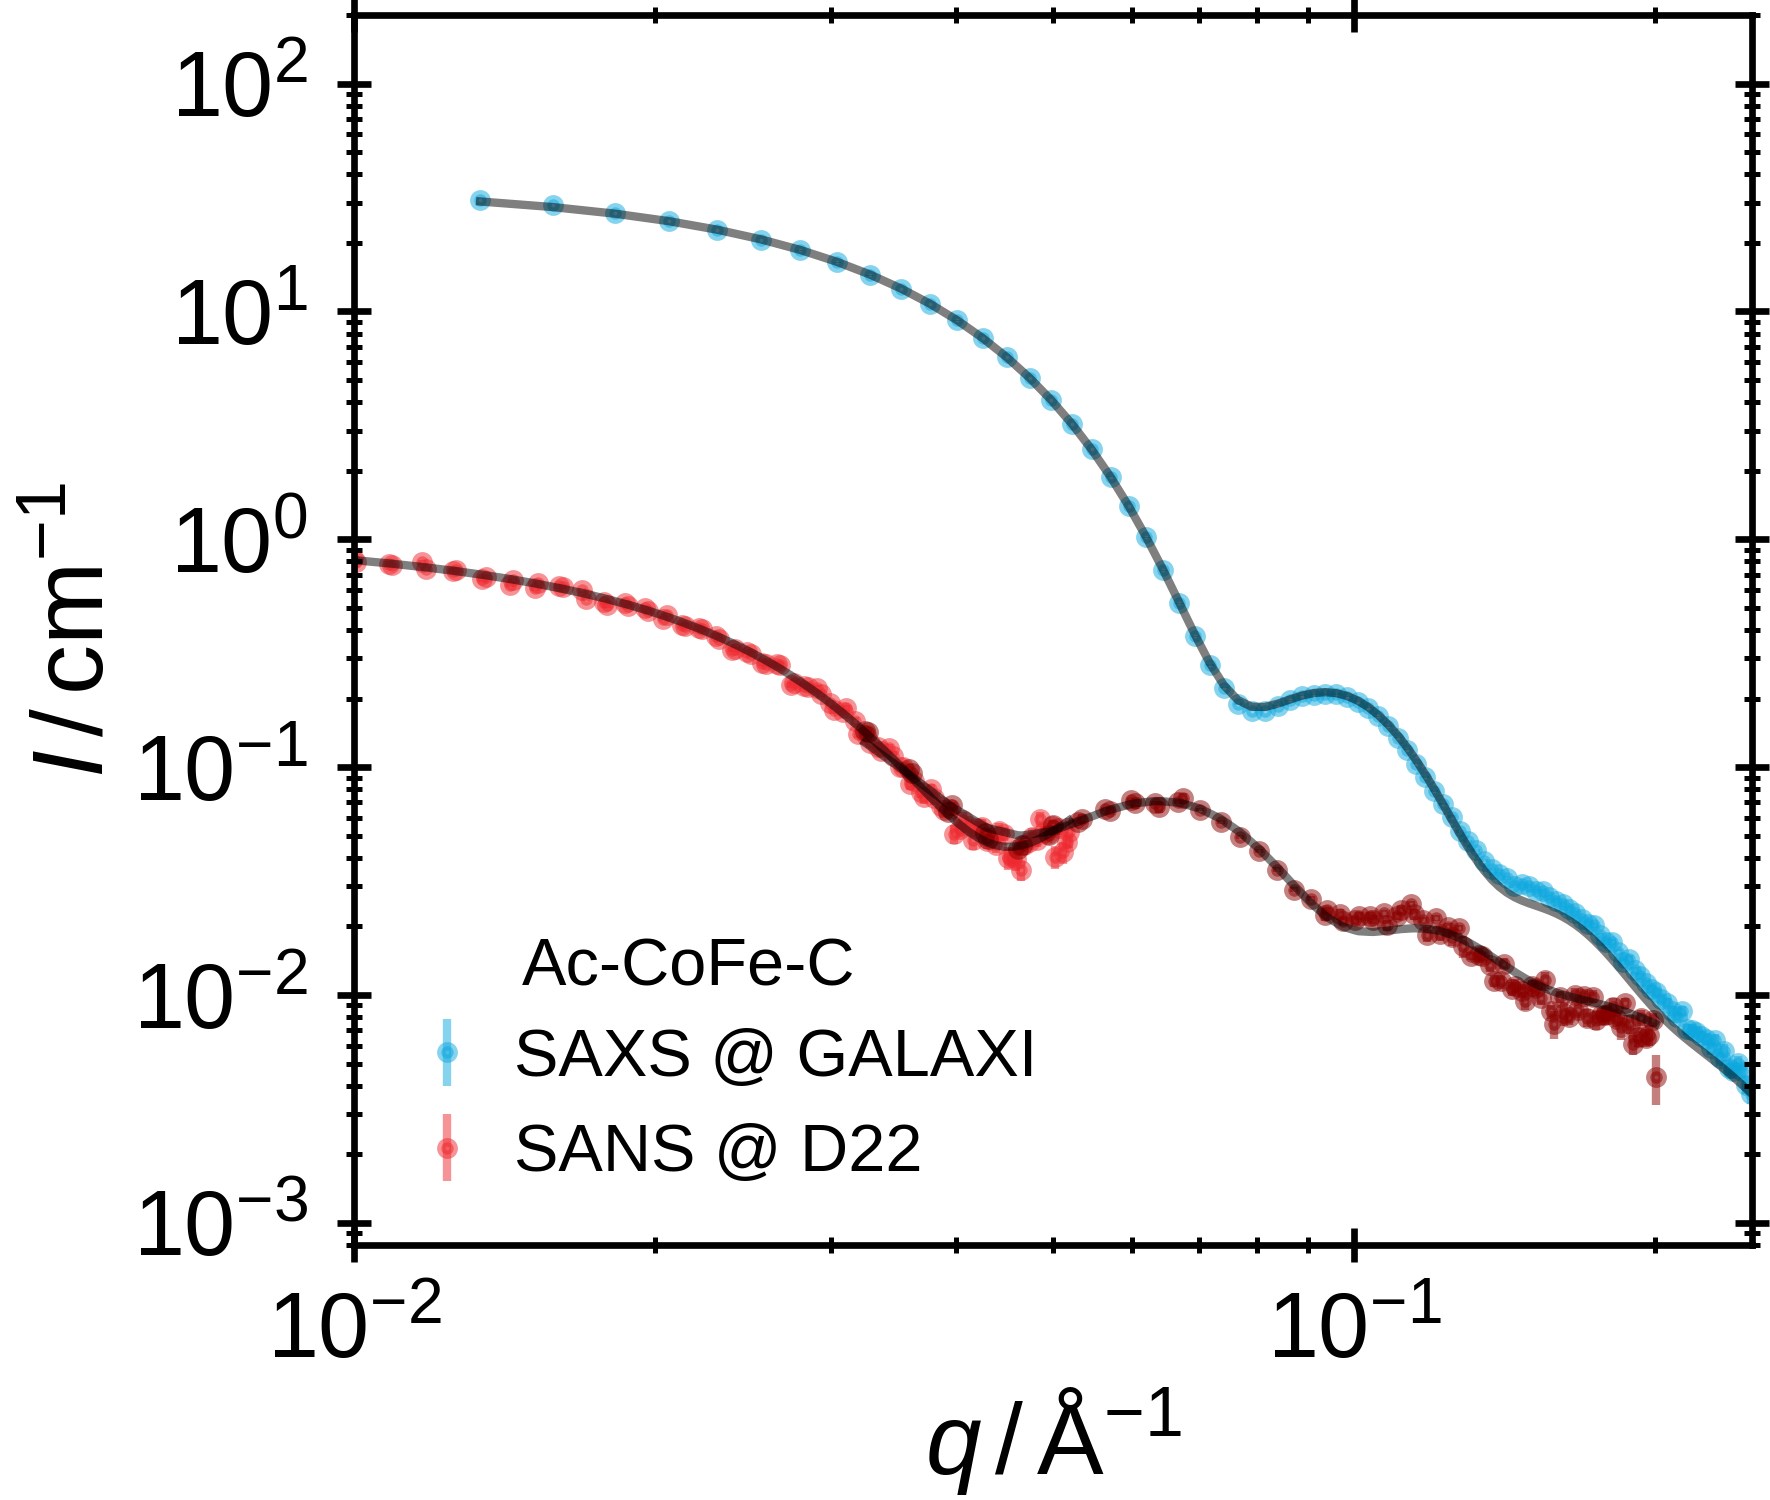
\includegraphics{monolayers_SAS_Ac_CoFe_C_SASFit}
      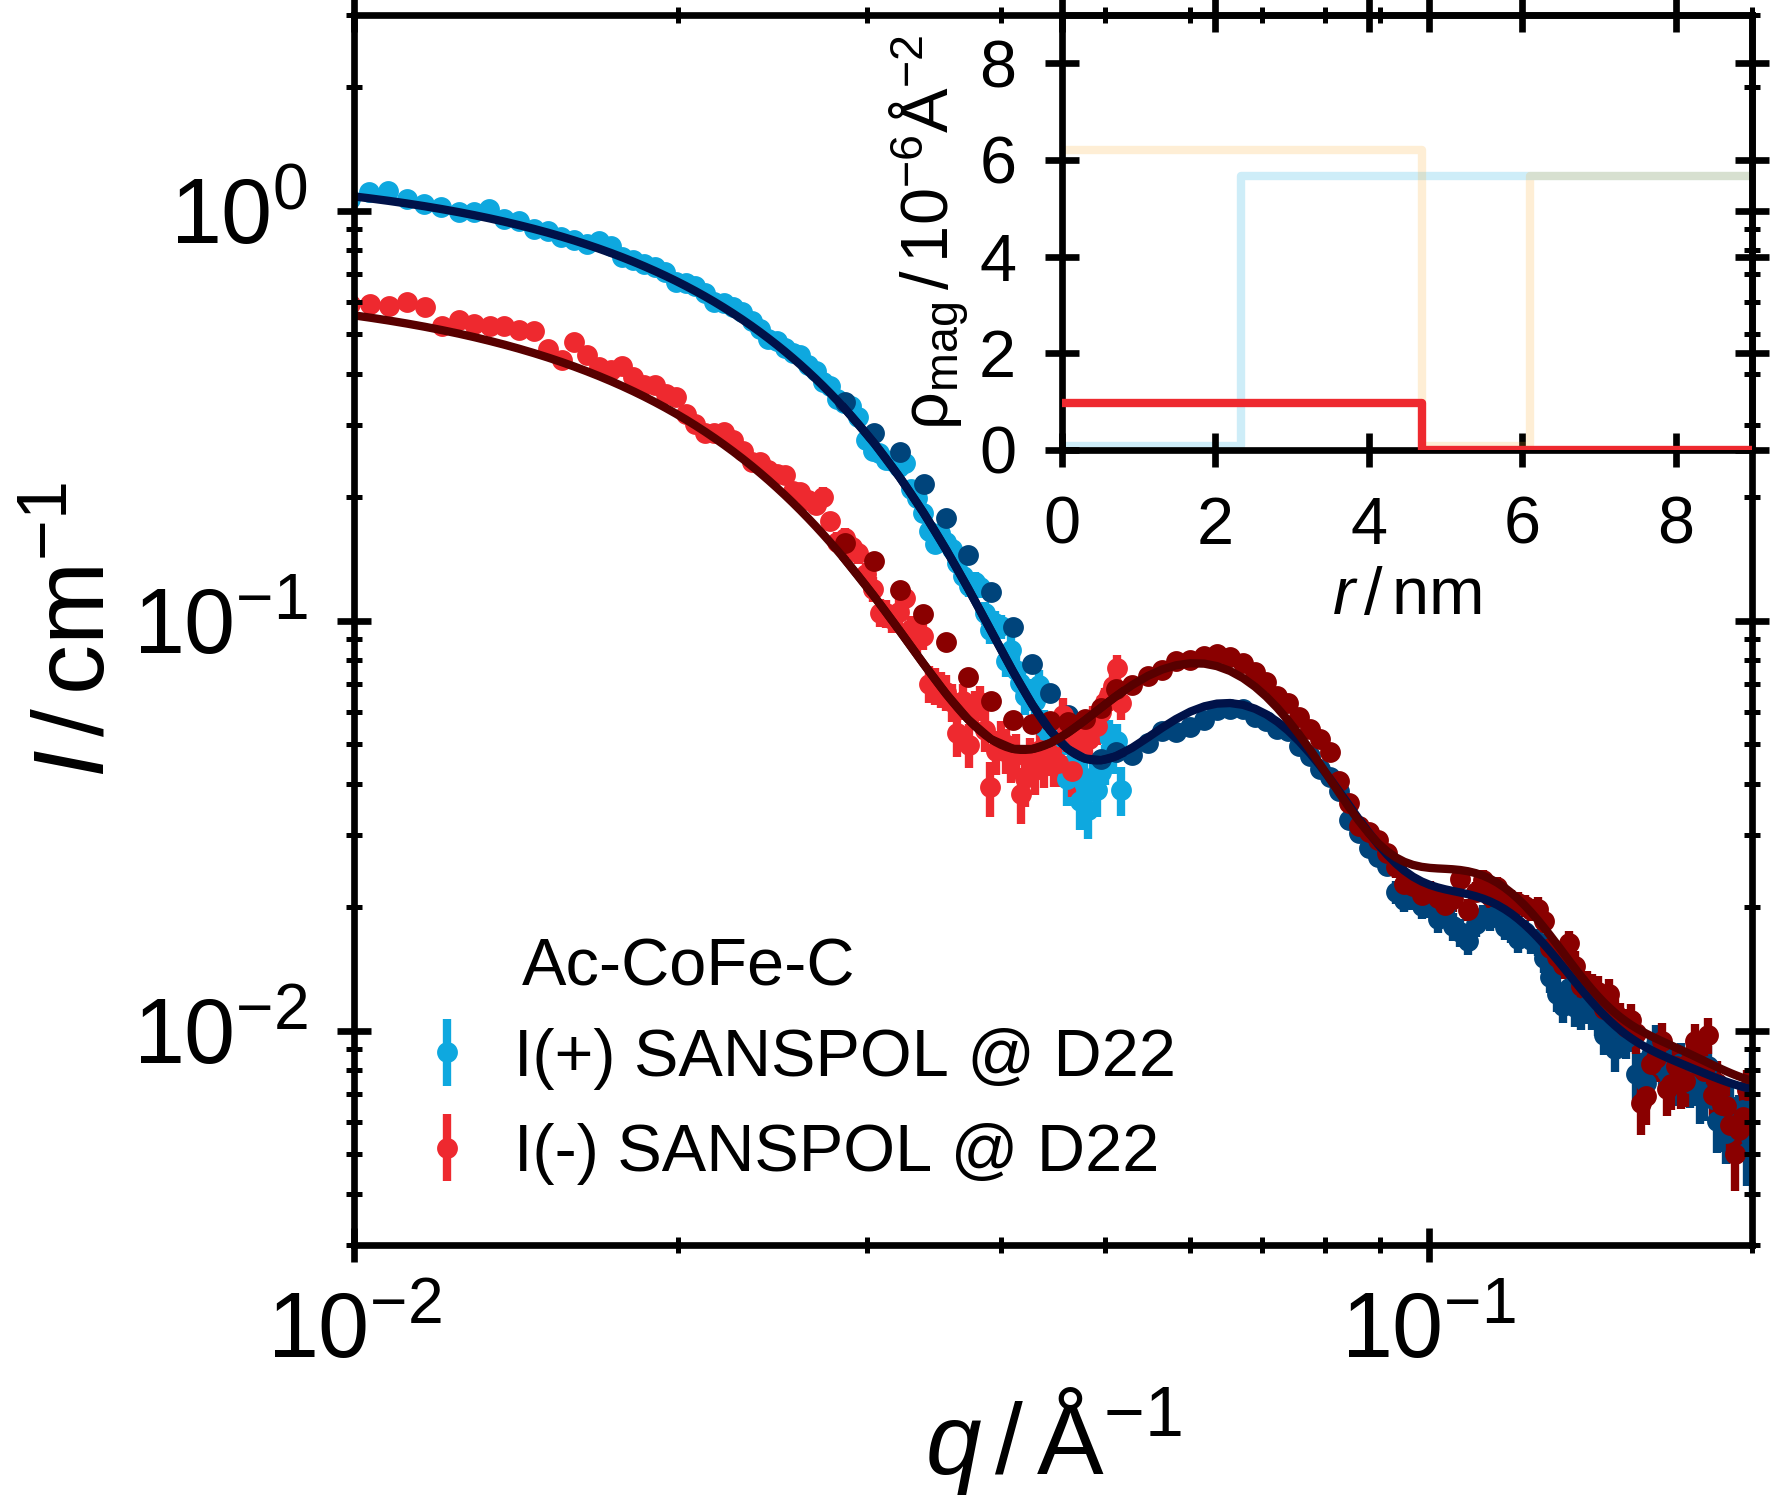
\includegraphics{monolayers_SAS_Ac_CoFe_C_SANSPOLFit}
      \caption{\label{fig:monolayers:nanoparticle:sas:AcOlCoFeC}SAXS and SANS measurement of Ol-CoFe-C (upper left) and Ac-CoFe-C (lower left), as well as SANSPOL at $1.2 \unit{T}$ respectively (right). The data is fit to a superball model.}
    \end{figure}

    To evaluate the data quantitatively, the data of both samples is fit with a superball model.
    Briefly, a superball is a mathematical shape that can be used to describe rounded cubes and it's defined by
    \begin{align}
      x^{2p} + y^{2p} + z^{2p} < R^{2p},
    \end{align}
    where $R$ is the radius of the superball and $p$ describes whether the body is closer to a sphere or a cube.
    For $p\eq1$ the superball is equivalent to the definition of a sphere and for $p \rightarrow \infty$ the superball converges to a cube with edge length $a \eq 2R$.
    The full description and derivation of the superball formfactor is described in \refapp{ch:appendix:numericalMethods:superballFormfactor}.
    The fitted model is shown in \reffig{fig:monolayers:nanoparticle:sas:AcOlCoFeC} and the important parameter of interest are given in \ref{tab:monolayers:nanoparticle:sas} for the following discussion, where the full set of model parameters is listed in \refapp{ch:appendix:modelparameters:monolayers:sas_olac_cofe_c}.
    \begin{table}[ht]
      \centering
      \caption{\label{tab:monolayers:nanoparticle:sas}Parameters of the superball fit of the small angle scattering data of the presented nanocubes, the complete set used to describe the models can be found in \refapp{ch:appendix:modelparameters:monolayers:sas_olac_cofe_c}.}
      \begin{tabular}{ c | l | l }
          & Ol-CoFe-C & Ac-CoFe-C \\
        \hline
        $R$
          & $5.62(2) \unit{nm}$
          & $4.29(4) \unit{nm}$\\
        $D$
          & $1.633(8) \unit{nm}$
          & $1.12(6) \unit{nm}$\\
        $p$
          & $1.54(3) \unit{nm}$
          & $2.2(2) \unit{nm}$\\
        $\sigma_R$
          & $9.27(8) \,\%$
          & $15.0(4) \,\%$\\
        $\rho_\mathrm{mag}^\mathrm{sans}$
          & $0.31(2) \cdot 10^{-6} \angstrom^{-2}$
          & $0.792(9) \cdot 10^{-6} \angstrom^{-2}$\\
        \hline
      \end{tabular}
    \end{table}
    The superball model result confirms the qualitative observation that the Ol-CoFe-C nanoparticles have a smaller size distribution than the Ac-CoFe-C cubes.
    Where the specimen size used to determine size and size distributions in transmission electron microscopy suggests a narrow size distribution for Ac-CoFe-C, the large number of particles scanned in the small angle scattering experiments reveals without bias that on average there is a greater variation in particle size.
    Furthermore, the model suggests that Ol-CoFe-C has a higher degree of roundness on the corners, visible from the small $p$ parameter.
    To verify this by local experiments, high resolution transmission electron microscopy (HR-TEM) experiments are necessary.
    A study comparing the effectiveness of the superball model in comparison to HR-TEM can be found in App. ??? for particle batches synthesized similar to Ac-CoFe-C.

    \begin{figure}[tb]
      \centering
      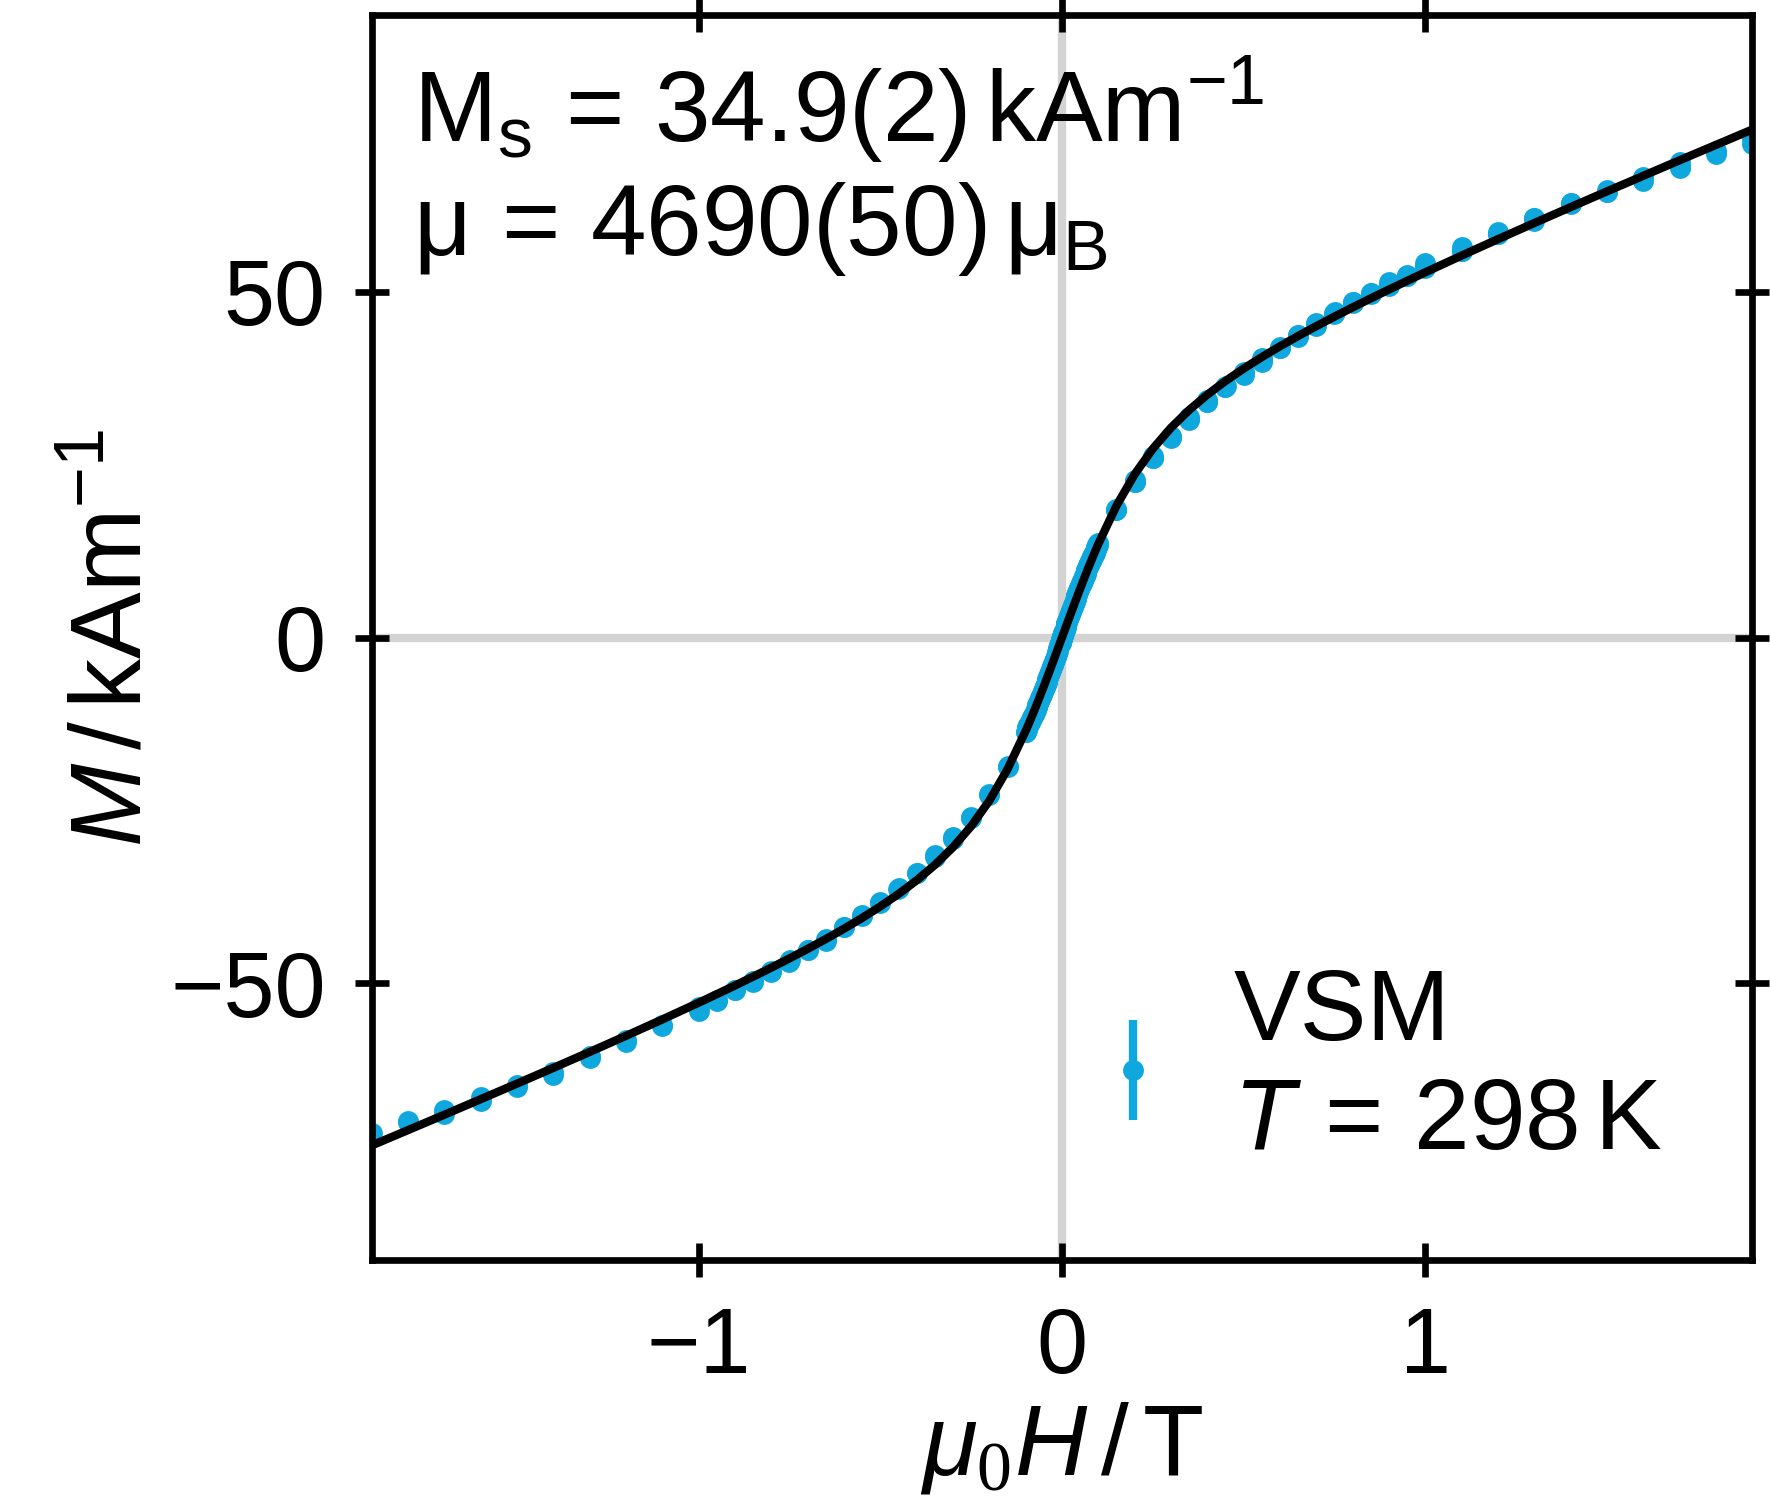
\includegraphics{monolayer_VSM_Ol_CoFe_C}
      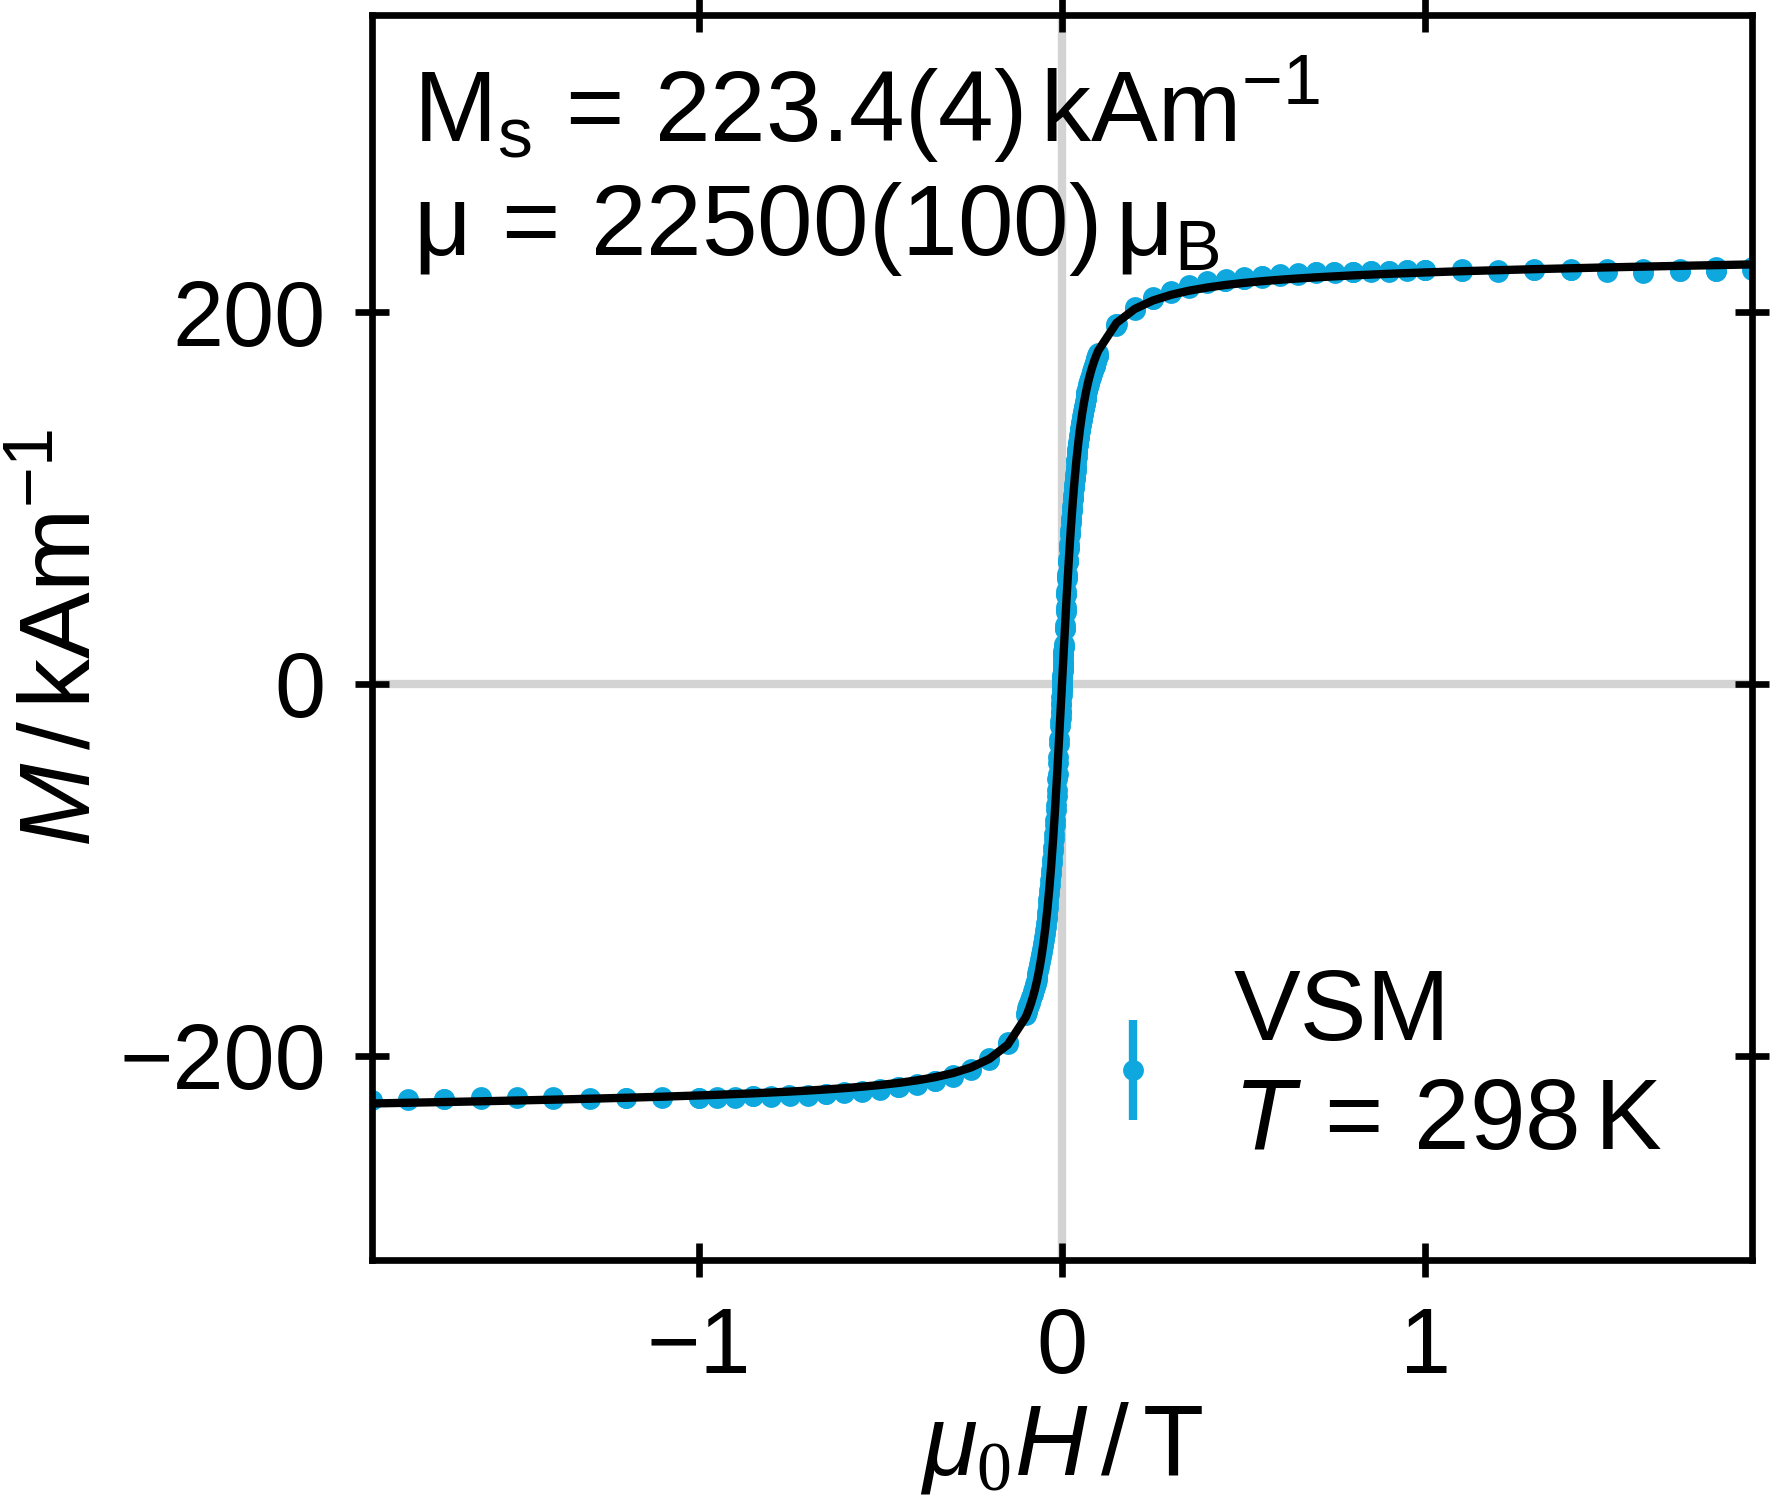
\includegraphics{monolayer_VSM_Ac_CoFe_C}
      \caption{\label{fig:monolayers:nanoparticle:vsm}Room-temperature hysteresis measurement of Ol-CoFe-C (upper left) and Ac-CoFe-C (lower left) taken on a vibrating sample magnetometer fitted with a Langevin curve.}
    \end{figure}

    From the SANSPOL data, the magnetic scattering length density is fit, which is used to determine the magnetization of the nanoparticle using \refeq{eq:looselyPackedNP:nanoparticles:SLDtoMagnetization} to $107(7) \unit{kAm^{-1}}$ for Ol-CoFe-C and $272(3) \unit{kAm^{-1}}$ for Ac-CoFe-C.
    This can be compared to the saturation magnetization obtained from measuring a liquid dispersions of nanoparticles on a vibrating sample magnetometer (VSM) as shown in \reffig{fig:monolayers:nanoparticle:vsm}, which results in magnetizations of $58 \unit{kAm^{-1}}$ for Ol-CoFe-C and $223 \unit{kAm^{-1}}$ for Ac-CoFe-C at the same magnetic field of $1.2 \unit{T}$.
    The discrepancy between the two results can largely be attributed to the difficulty in measuring liquid samples in a vibrating sample magnetometer and determining the volume of the magnetic material for the normalization of the VSM data.
    When liquid samples of nanoparticles are measured in a VSM, one assumes that the particle perfectly follow the vibrating motion exerted on the liquid like a solid sample would.
    However, due to inertia and finite viscosity it can be assumed that the particle motion is lagging the vibrating motion and therefore that the signal strength might be off.
    And on the other hand, the presented data is always scaled to the assumed total volume of magnetic material in the sample, which is estimated for a nanoparticle dispersion from the particle mass concentration of the dispersion.
    Due to both reasons, the quantitative comparison of VSM and SANSPOL data might be off.
    But importantly, on a qualitative level, both experiments agree in the result that the nanoparticles from the oleate route are weakly magnetic, while the particles from the acetylacetonates are strongly magnetic.

    \begin{figure}[tb]
      \centering
      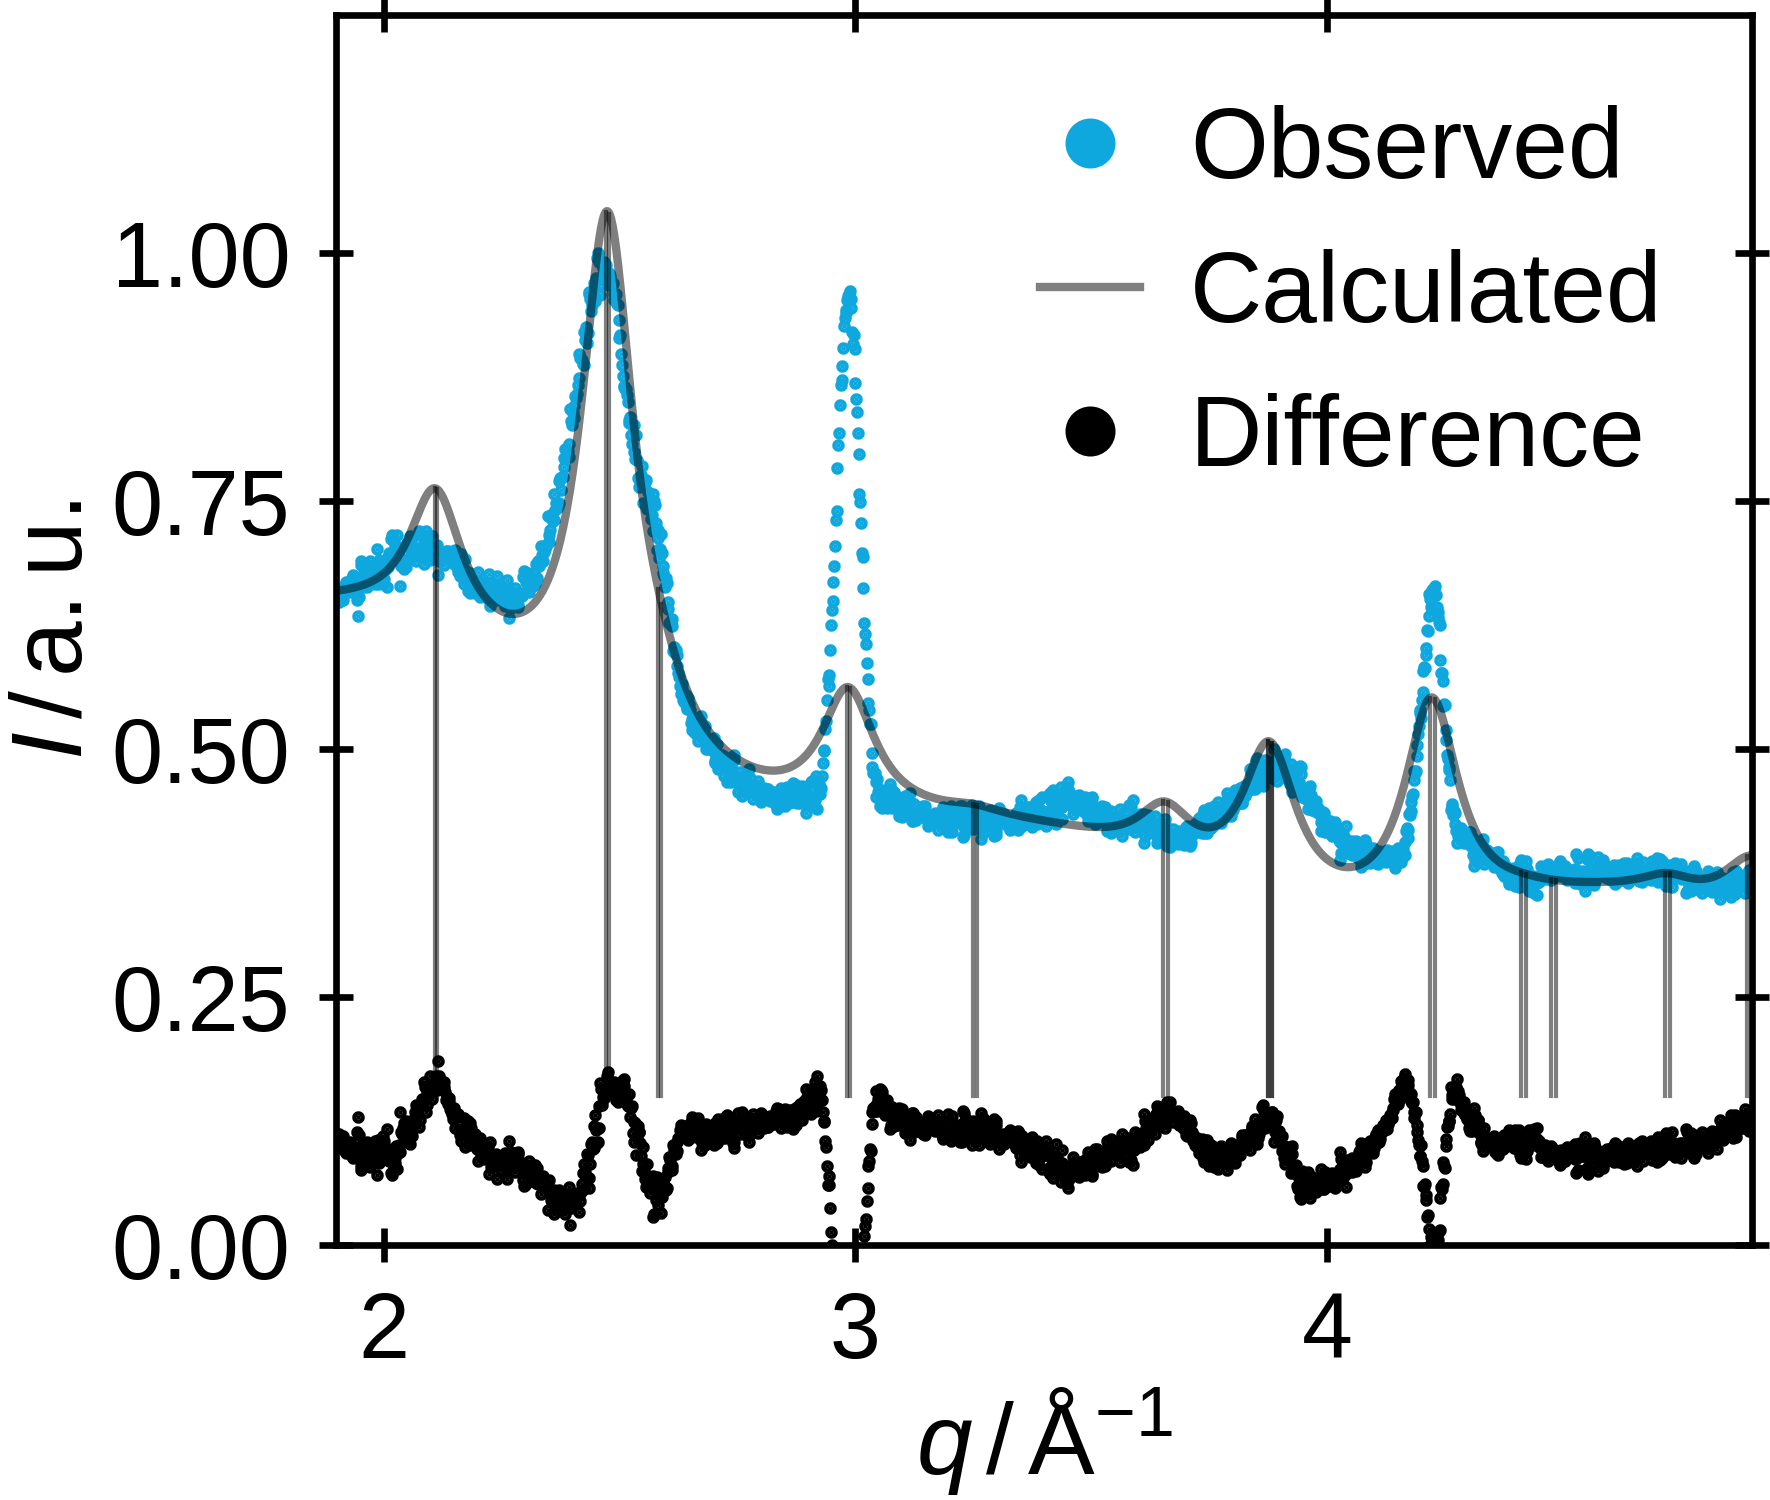
\includegraphics{monolayer_XRD_Ol_CoFe_C}
      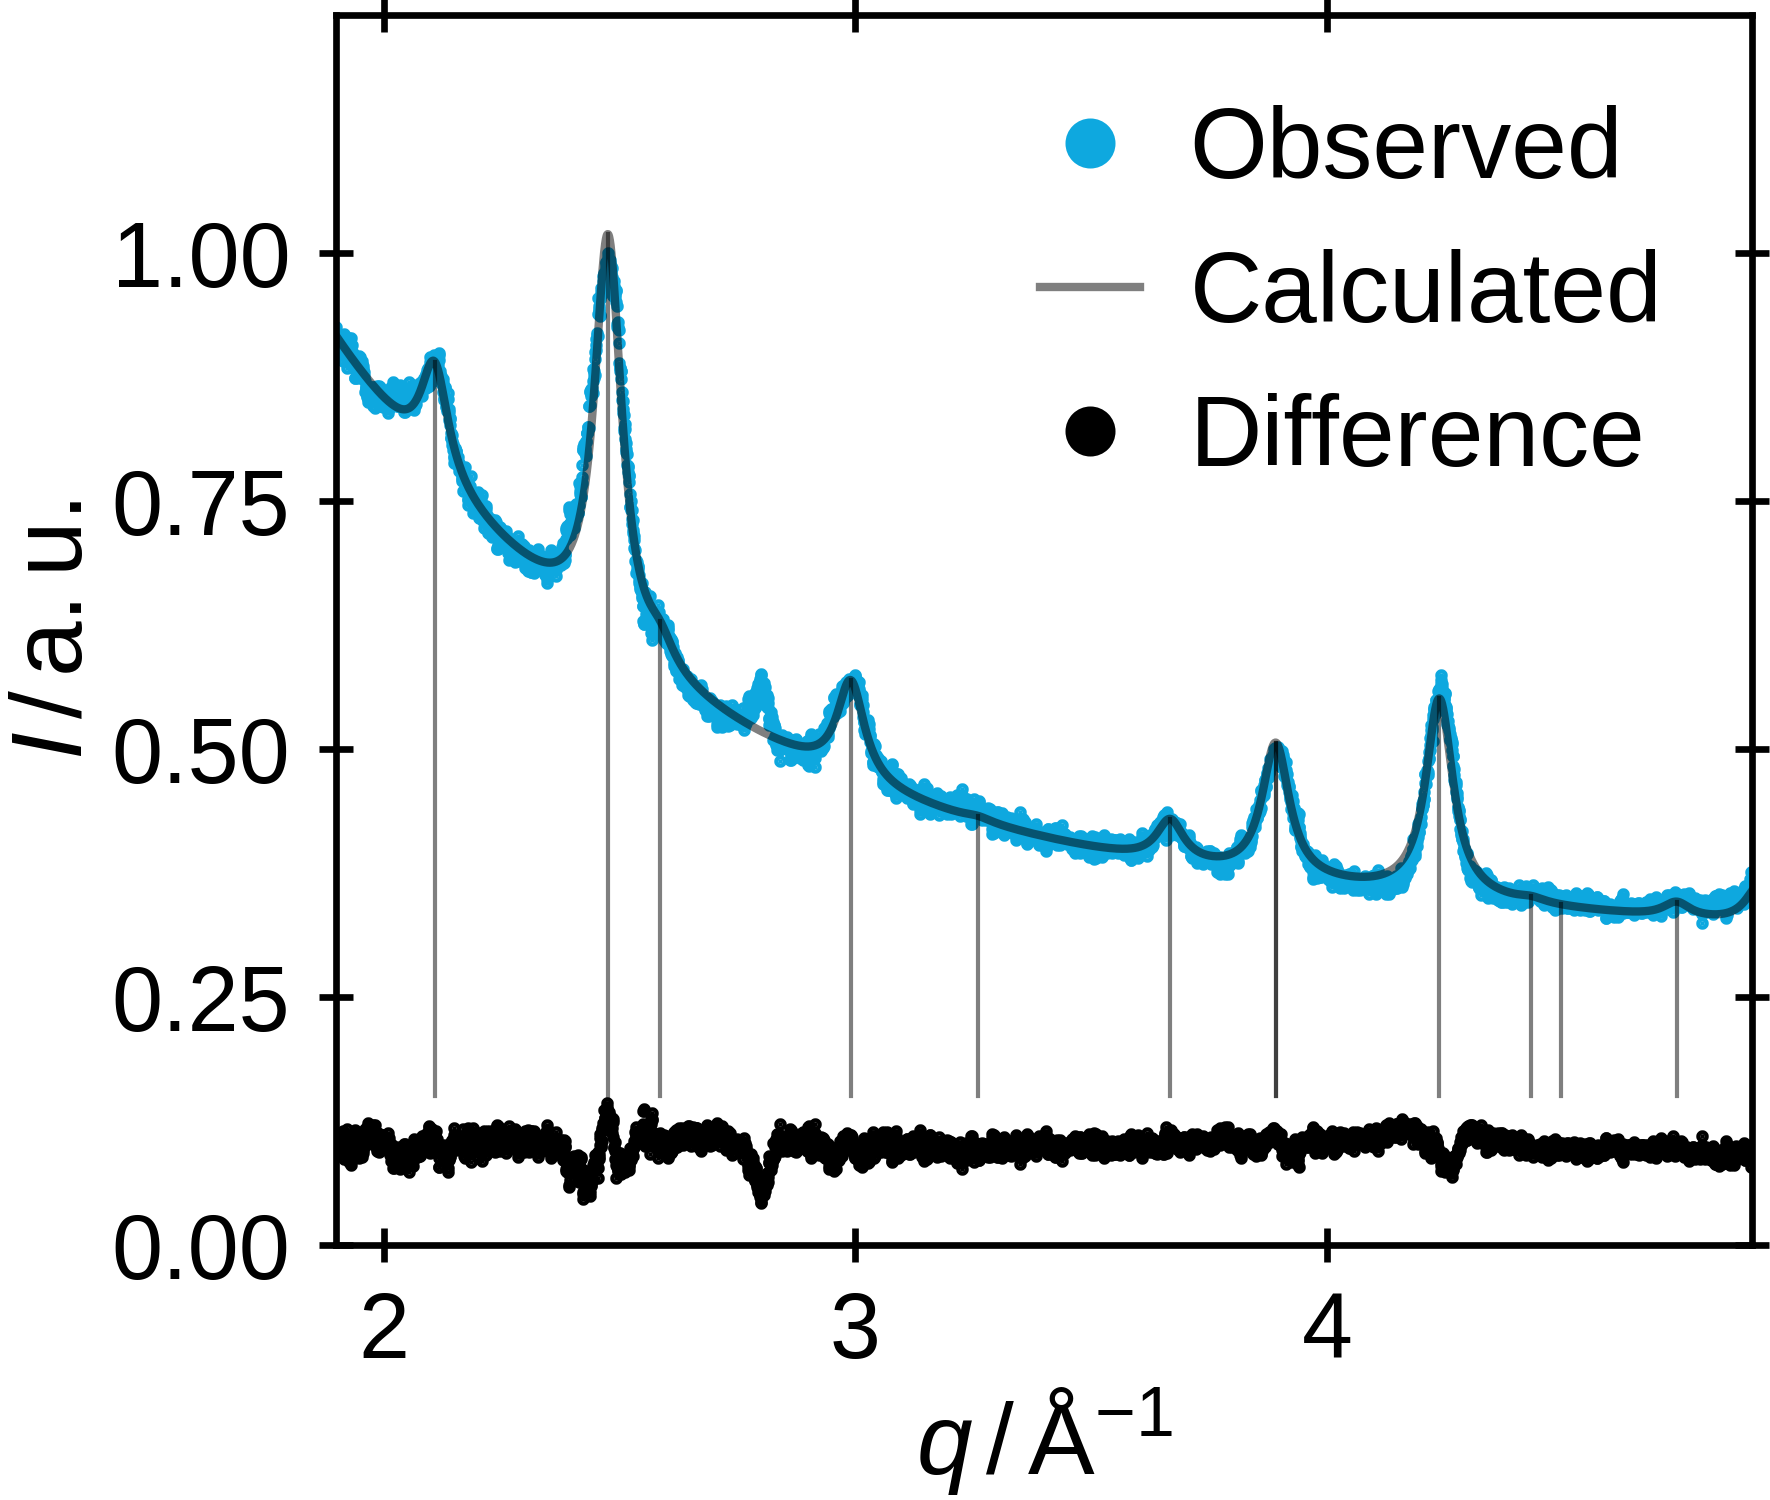
\includegraphics{monolayer_XRD_Ac_CoFe_C}
      \caption{\label{fig:monolayers:nanoparticle:xrd}X-ray diffraction of Ol-CoFe-C (left) and Ac-CoFe-C (right) with a Rietveld refinement assuming an inverse spinell structure.}
    \end{figure}

    An explanation for the weak magnetic properties of the oleate synthesized particles is found in literature and confirmed when looking at X-ray diffraction data as shown in \reffig{fig:monolayers:nanoparticle:xrd}.
    Where the particles from acetylacetonates are well fitted by the inverse spinell structure, which one expects for cobalt ferrite, Ol-CoFe-C deviates strongly from this.
    The peaks are visibly broadened in comparison, the relative intensities of the peaks do not match and an additional peak around $q \eq 3.5 \unit{\angstrom^{-1}}$ is visible.
    Earlier works on nanoparticles synthesized from oleates \cite{Bodnarchuk_2009_Excha, Wetterskog_2013_Anoma} report already that instead of pure phased cobalt ferrite particles, core-shell particles with an antiferromagnetic w\"ustite core are obtained during the oleate synthesis due to the reductive environment of the synthesis.
    And indeed, including a w\"ustite phase in the Rietveld refinement greatly improves the model as shown in Fig. ??.

    \begin{figure}[tb]
      \centering
      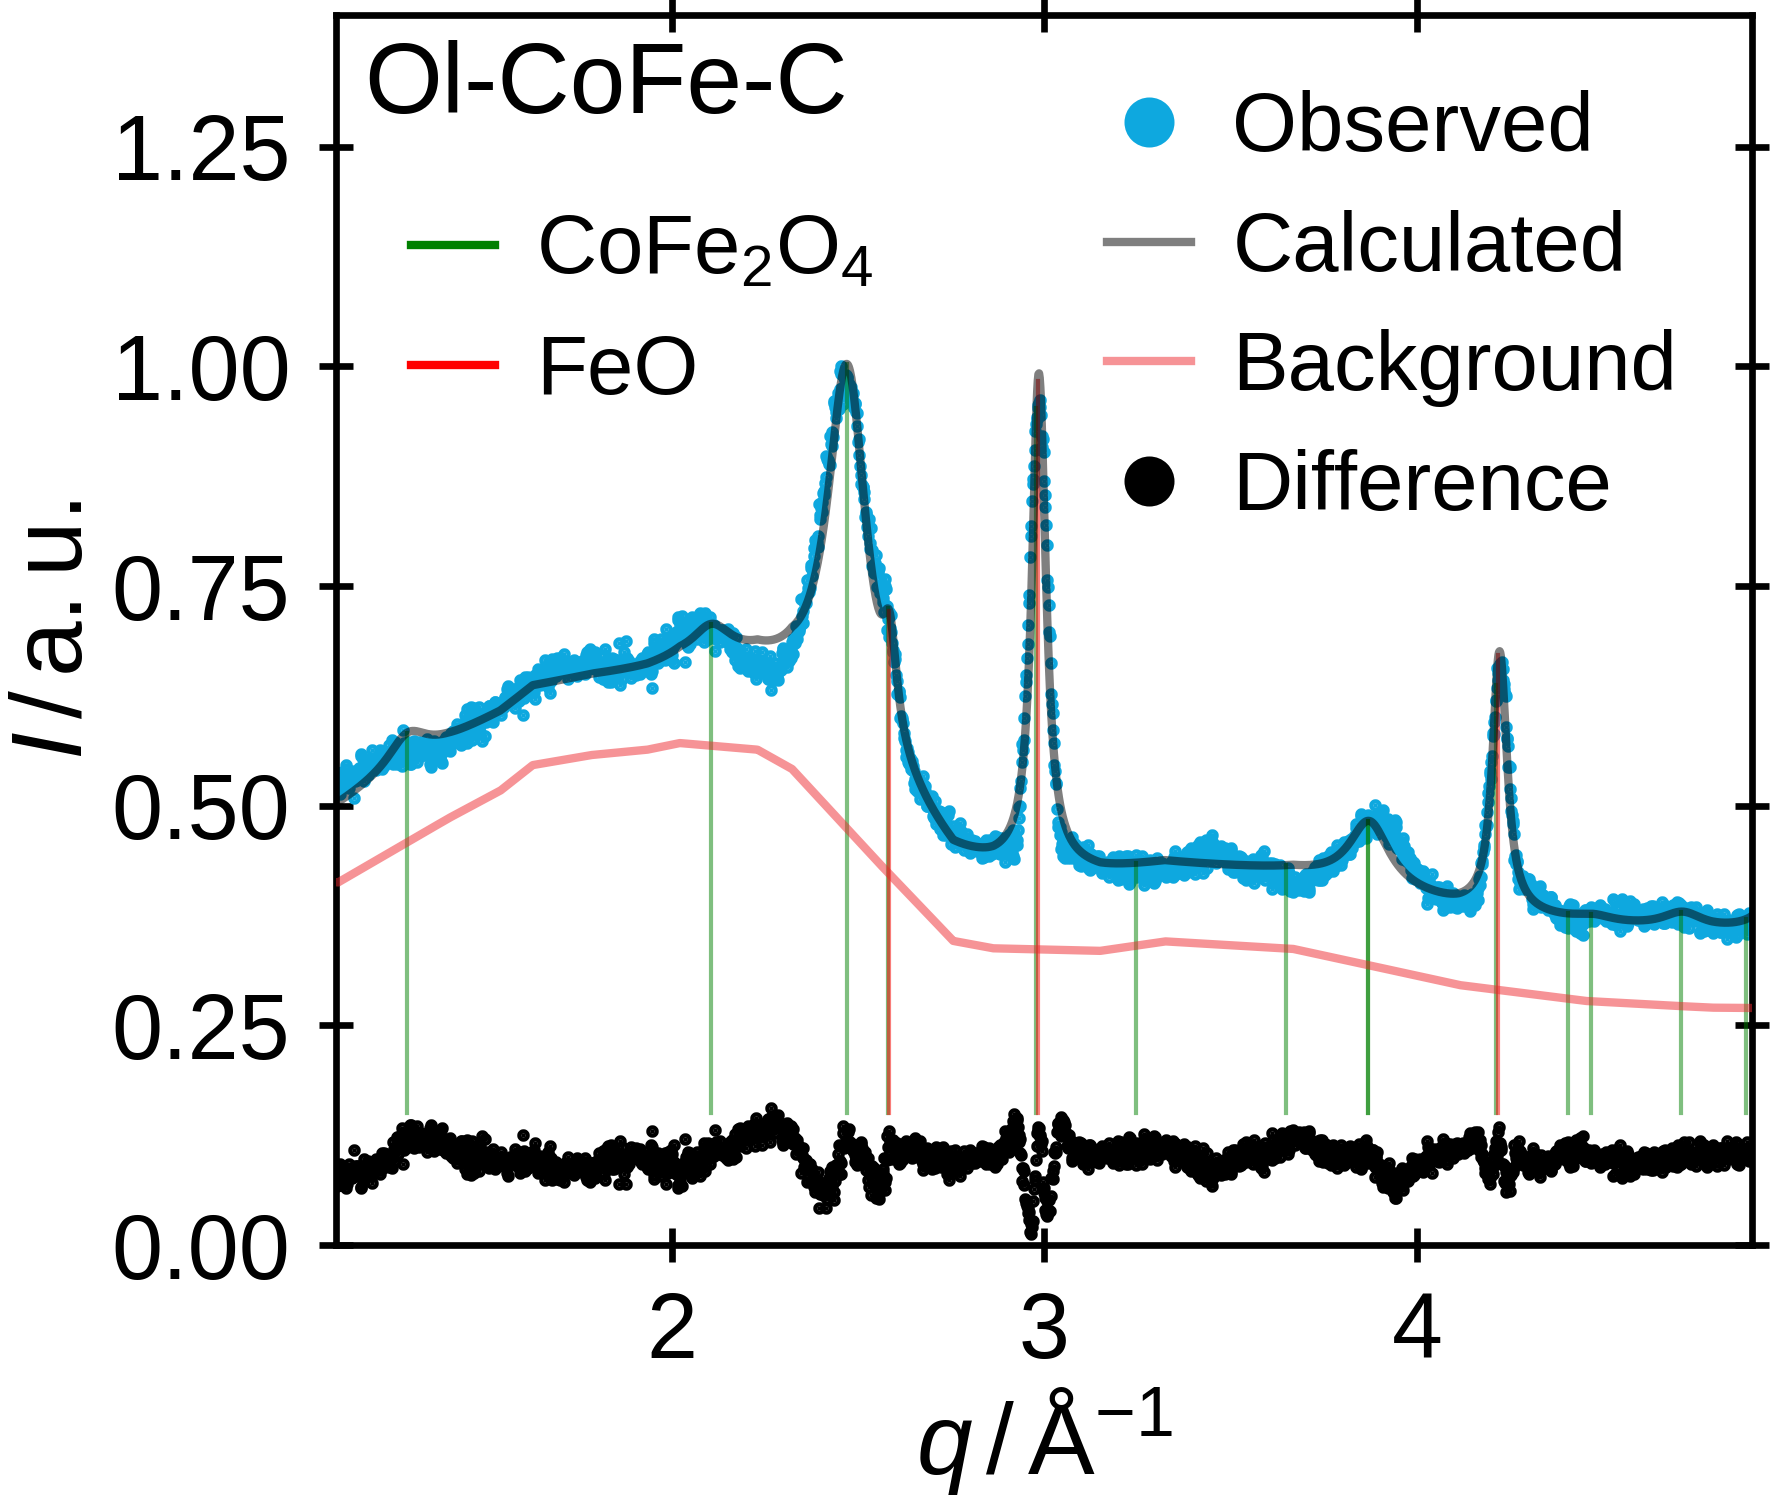
\includegraphics{monolayer_XRD_CoFe2O4WustiteFit_Ol_CoFe_C}
      \caption{\label{fig:monolayers:nanoparticle:xrd}X-ray diffraction of Ol-CoFe-C with a Rietveld refinement assuming a combination of cobalt ferrite and w\"ustite.}
    \end{figure}

\end{document}